%!TEX root=../tax-n-democracy-held.tex

%Some kind of introduction, what are those bumps?
%they are interlinked

%overall quote

\chapter[Three Crises]{A Tale of Three Crises} \label{chap:3-crises}

%the headings in the below stink

\section{The Crisis of the Welfare State}

\begin{quote}
	\emph{``Private affluence, public squalor.''}\\*
	--- John K. \citealt{Galbraith1959}
\end{quote}

%cite some Butterwegge work on inequality
%cite some Groh-Samberg work on inequality

	%Baumol explicitly endorses tax hikes to make sure that cost disease doesn't cause public squalor \cite{Baumol1992}
	
	%note that much of the economics in here are what is known as "comparative statics"

\subsection{Excessive Inefficiency is Inequitable} \label{sec:InefficiencyIsInequitable}
Equity and efficiency, at the extremes, are not as conceptually orthogonal as conveniently assumed: Excessive inefficiency is, in fact, likely to be inequitable, too, as government failure to provide public goods and pool risks has a social gradient. Poorer individuals will be hit harder, because public goods and lemons markets are not, in truth, dichotomous and uniform phenomena. In the real world, some public goods (for example, policing) have close, if costly private good substitutes (for example, gated community). Similarly, some risks will be more symmetrically observable (for example, buyers of private health insurance in Germany tend to be better and better-known risks). Alternatively, rich people may have enough assets to forego risk pooling alltogether (for example, excessive co-payments). In short, rich people can often buy their way out of otherwise underfunded or failing public institutions, creating yet greater inequities \citep{Barry2002}.

%Moreover, inequality and common/public goods and risk pooling are not as distinct concepts as presented in the above table, when taken to the (reasonable) extreme and adding a dynamic dimension. 
%
%Inequality is, in the above assumed to be a policy challenge in its own right, that calls for \emph{redistribution}. Alternatively, from a more dynamic perspective, gross, self-reinforcing inequities could also be framed as public or common good problems, where excessive inequality exerts a negative externality of non-opportunity on the poor. Taking things further into the future, presently existing inequality could be assumed to exert a negative externality on the future, forgoing otherwise more broadly-based growth.
%
%Conversely, excessive underprovision of common/public goods or a lack of effective risk-pooling easily hits the poor hardest, who have few other resources to buy or substitute the lacking goods.
%
%Policy makers should, however, be careful not to introduce duplicate redistributive mechanisms in other state activities, such as Pigouvian taxes or fees, which are not geared towards everyone, but a certain type of behavior or service consumed. 
%
%A further requirement of ``regulatory neatness'' and corrolarly of this thinking is that redistributive and revenue-generation taxes should in principal be levied on natural persons exclusively. Only between natural persons is redistribution meaningful, even ignoring the above-mentioned problems of incidence and uniform progression discussed in the above. 

\subsection{Excessive Inequality is Inefficient}
\label{sec:InequalityIsInefficient}
Equity and efficiency are not a zero-sum trade-off. Sometimes, when the cake is sliced up more equitably, it may grow. Formulations of such positive-sum relationship between the two vary, and only some examples can be given here.

%also cite here the Jacobs mathematician \cite{Lorenz2013} et al who seem to have done some kind of portfolio modeling to show the same thing. this is about human capital. get into this. this might belong somewhere else.

%note (this is from somewhere, either Cassidy or Frank, probably frank, that more equality can make more Coase-style deals happen; that's what you want, be it in Coase-style property rights or Pigovian taxation. You don't want: having distributive stuff kreep into commons et al. Good example: Pendlerpauschale in Deutschland. This is an important point, I think this also works with only the harms principle as justification. Don't let go off this point.
	%Argue: It's always better to have coase-theorem style exchanges on common goods rather than to regulate them (also: exernalities), examples including airplane tickets when they're overbooked, it's no longer first-come-first-serve, but you get a compensation for volunteering (auctioned off). %idea from robert frank on the dawin economy. Re-read ch 6 on the coast theorem and in paying for public goods.
	%The thought is this, beginning in chapter 8: if there's income economy inequality the demand for public goods is likely to decrease, because willingness to pay differs greatly between different users of the public good. Example: public goods costs 1000$, equal use for 2 people, but b/c of very different incomes, their willingness to pay is 900 and 200, and so it's not happening maybe.
	%This is interesting, because, here's a Caplan-Style political economy (all cost benefit), and even THIS is plagued by income inequality. If you have lesser income inequality, this decision even in a caplan world would work.

\subsubsection{Structural Unemployment} \label{sec:StructuralUnemployment}
%instead of structural unemployment speak of natural unemployment, which is frictional PLUS strucltural (unions, min. wages, efficiency wages/aka reserve army). Opposed to this is cyclical unemployment

Extreme inequality in post-tax market outcomes may also conflict with the efficiency goal of full factor employment. Most (post)industrial societies have legislated socially accepted minimal incomes. This legislation takes the form of statutory minimum wages or unemployment benefits. Either way, an effective or de-facto price floor for wages is established\footnote{Income subsidies or negative income taxes may not lead to such dysfunctional price floors (\hyperref[http://maxheld.de/2010/04/19/sharing-the-burden/]{c.f.} \citealt{Held2010}).}. People with productivities \emph{below} this price floor will not find employment, leading to a DWL of structural unemployment\footnote{I assume here that market wages are low \emph{only} because of low productivities, in keeping with \hyperref[sec:PerfectCompetition]{perfect competition} condition {itm:PriceTakers} (\hyperref[itm:PriceTakers]{infinite buyers and sellers}). If, by contrast, employers have great bargaining power over non-unionized workers (as appears to be the case in much of the service sector) they may receive low wages even when their labor productivities are adequate. Such Manchester-capitalism styled exploitation should be met with regulatory, not fiscal interventions: otherwise, government may end up transferring to exploitative firms.

It does not matter \emph{why} labor productivity of some groups of workers is in \emph{relative} decline. Candidate culprits include international trade and finance (for example, discredited \citealt{Stolper1941}) as well as skill-based technological progress \citep{Card2001}. Whatever the reason for low relative labor productivities, an efficient fiscal configuration should help factor markets clear.}.

Crucially, the level of minimal incomes depends on the broader configuration of tax incidence, indirect taxes in particular. When taxes are relatively flat and fall on labor or consumption, the real costs of living for low-income earners rise. This \emph{tax wedge} can take the form of (flat or proportional, payroll-style) social contributions, VAT or a relatively flat or proportional personal income tax: either way, \emph{more} money has to be made on the market for the same living standard (in Purchasing Power Parities, PPP).

The implications for tax design are twofold:

\paragraph{Structural Unemployment as Endogenous.} 
The only genuine fix to structural unemployment is of course more education to lift people, or at least their children, out of their low standards of productivity. Better education, to be sure, will require fresh ideas --- but also lots of public resources. Well-funded public education, in turn, is endogenous to a fiscal configuration (compare \autoref{sec:Underqualification} on the \hyperref[sec:Underqualification]{real dissaving of underqualification}).

\paragraph{Structural Unemployment as Exogenous.} 
Even from a static perspective, assuming low-productivity workers to be exogenous, some measure of tax relief for would-be working poor may enhance welfare. An efficient tax system should reduce the burden on low-productivity earners, to keep their post-tax socially acceptable minimum wages as low as possible. 
\newpage
\begin{desideratum}[Low Cost of Living for Low-Productivity Earners]
	A desirable tax has a minimal incidence on low-productivity earners to lower their cost of living.
	\label{des:low-price-floor}
\end{desideratum}

\subsubsection{Excessive Inequality Squanders Talent.} 
Extravagant inequalities that bear no meaningful relationship between effort and reward squander talent as Malcolm \citeauthor{Gladwell} argues in \emph{Outliers} (\citeyear{Gladwell}). This pop-sociological debunking of the meritocratic myth resonates with needs 
	%style!
for a large and highly qualified workforce, and concerns of social immobility in (post)industrial economies (for example, Lisbon Strategy, EU 2020). For a knowledge economy, you need lots of qualified and motivated people, not just a few stars.

\subsection[Heterogeneity]{Heterogeneity: The Sources of Wealth} \label{sec:sources-of-wealth} The \gls{EU} is a union of very unequal member states. On of the richer large member state, France (\$ 44,747 nominal \gls{GDP} per capita according to the IMF 2010) is six times richer than the poorest member state, Bulgaria (\$ 6,334 nominal \gls{GDP} per capita, \emph{ibid.}.). Within \gls{EU}-15, Luxembourg's \gls{GDP} per capita in \gls{PPP} was 3,5 that of Portugal. Within \gls{EU}-27, that multiple has widened to 7,4 times Luxembourg and Bulgaria (\citealt{Alber2008}: 1). %add gini, other union level statistic?

%capital formation is a better term than accumulation

Why this difference?

\paragraph{Productivity} The wealth of nations, as Adam \cite{Smith-1776-lq} taught, ultimately depends on labor productivity. Both nations and people prosper when they can get much out of the ultimately scarcest resource, human effort. 

This labor productivity, as \gls{GDP} per capita, varies widely between rich (for example, France 116) and poor (for example, Bulgaria 41.3, both in 2010, indexed to EU-25 average, Eurostat 2010)\footnote{
	Current labor productivities, as \gls{GDP} per capita probably understate the discreptancies. They are both after (much) regional integration. Without trade and investment --- ex-ante EU membership --- domestic economic output might be much lower still.}. 
Labor productivity, in turn, depends on technology (\gls{TFP} or Solow residuals), human capital (skills) and stocks of physical capital (for example, factories). These achievements, tangible or not, are all past surplus production coagulated into some form of capital. At some point in the past, someone had to have an extra bit of time or food on her hands to build something lasting, above and beyond subsistence consumption.
	%TFPs and Solow Residuals are important!

%financial intermediaries are: banks, funds, insurance. They do different jobs. For financial paper: these products and intermediaries are great, they do great things.


Why does it matter?

\begin{enumerate}
	\item Because capital is transformed surplus production, it is always an inheritance from the past. And so, much of current output depends on past capital accumulation and its historical circumstance in geography, geology, culture and political institutions. It matters a great deal, which circumstances encourage saving and innovation, but that question need not concern us here. %add link saving

	However, we need to remember here, that current performance is \emph{not} sufficiently linked to current output. Romanian workers at Dacia, a car manufacturer, produce less value in an hour primarily \emph{not} because they are lazier or sloppier, but because Romania lags in capital accumulation and cannot provide them with the skills and machinery that their French counterparts at Renault have. 

	\item Because capital is transformed surplus production, differences in output between people, countries and regions are here to stay, at least for some time.
\end{enumerate}

%more stats are here: http://epp.eurostat.ec.europa.eu/tgm/table.do?tab=table&init=1&plugin=1&language=en&pcode=tsieb030, 

I now discuss some broad economic dynamics likely operating on this partially integrated, and enormously heterogeneous economy. 

%money is: medium of exchange, unit of account and store of value. It can be either commodity money (intrinsic value), or it can be fiat (paper, paypal, bitcoins). The money stock is very difficult to know because the definitions are vague.

%The result of the two crises is an economy with runaway inequities, foregone productive capacity and a suboptimal net savings rate, in the face of greater challenges ahead (for example, aging, global warming).

%First, developed welfare states, in spite of their unprecedented prosperity, appear to be increasingly constrained in their ability to raise revenue and redistribute it as their legislators see fit. 

%Structural underfunding is caused by a state that is increasingly unable to raise sufficient revenue necessary for the provision of risk pools, public and common goods, as well as to finance its allocative goals.

%The result of the two crises is an economy with runaway inequities, foregone productive capacity and a suboptimal net savings rate, in the face of greater challenges ahead (for example, aging, global warming).

 \begin{figure}[htbp]
	\centering
	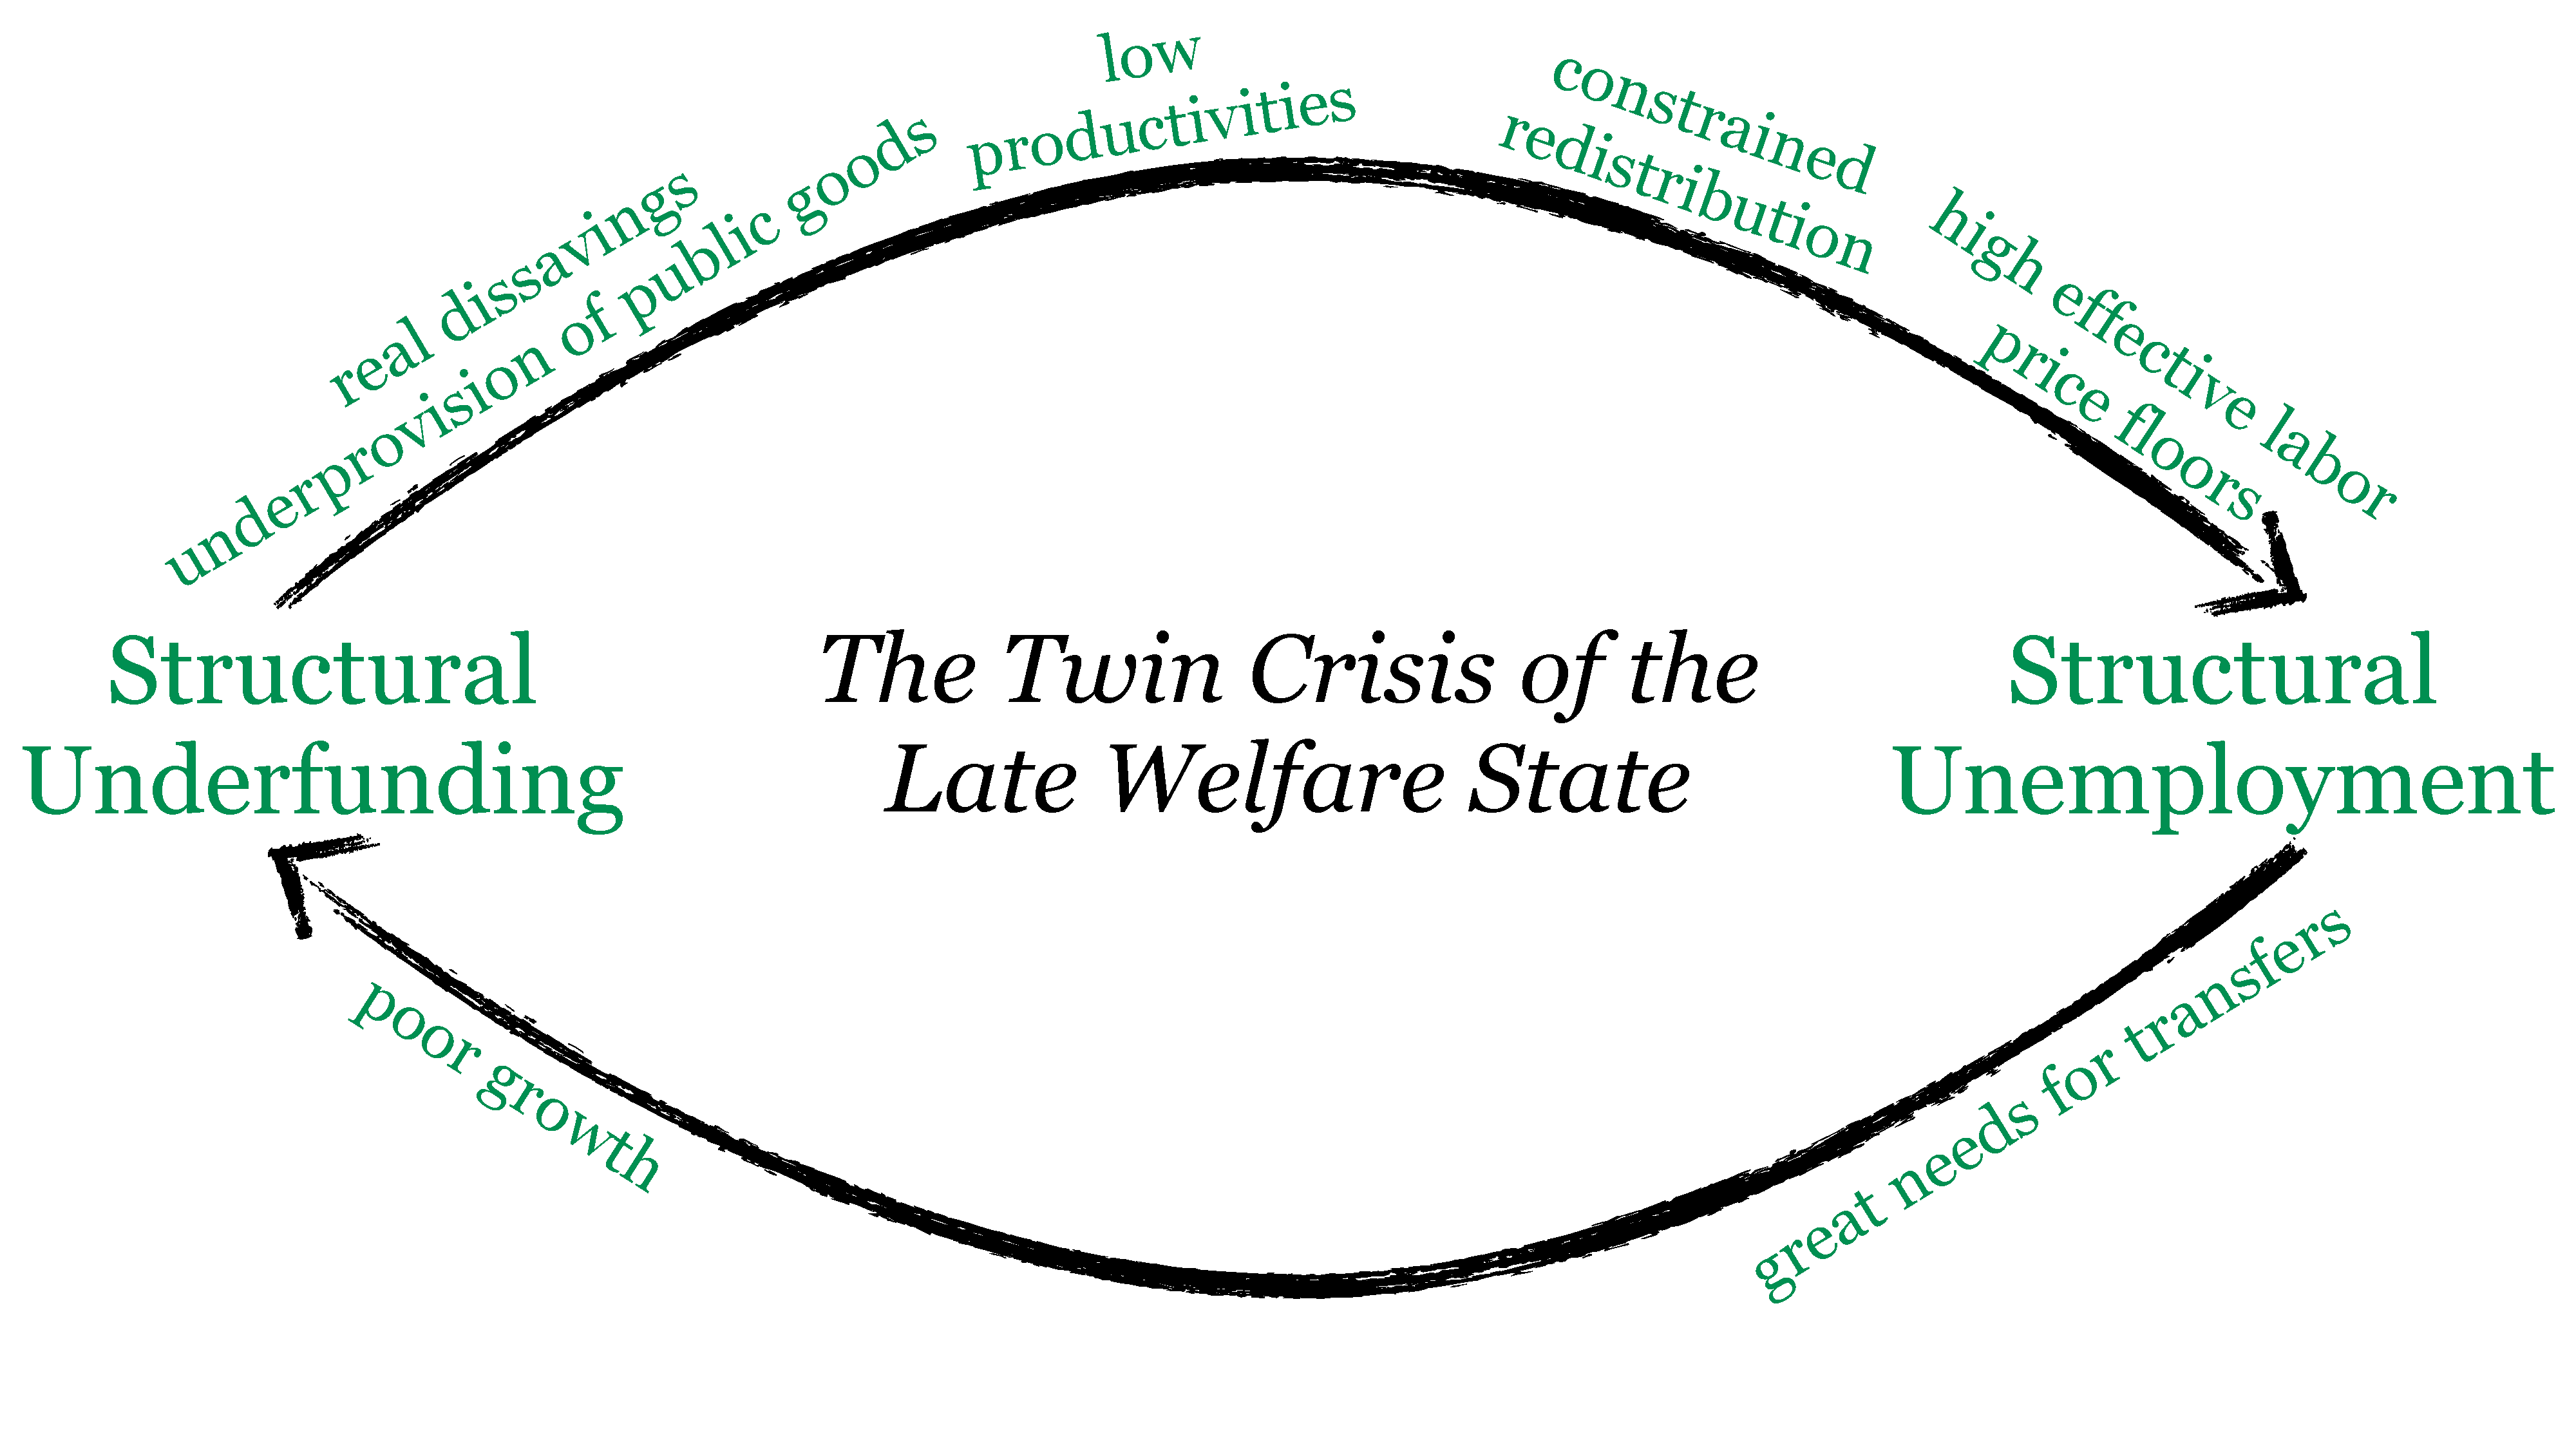
\includegraphics[width=1\linewidth]{dual-crisis}  
	\caption{The Dual Crisis of the Late Welfare State}
	\label{fig:dual-crisis}
\end{figure} 

%Today, welfare states are challenged or changed on a number of fronts. Internally, welfare provision is challenged by aging societies in the developed world, with resulting higher dependency rates and costs under “pay-as-you-go” systems (Castles 2002). Moreover, revenues and costs are affected by prolonged and extensive macroeconomic disequilibria, especially structural unemployment (which of course, can also be an effect of inadequate welfare regime design). Decreasing rates of productivity and output growth have heightened concerns, and de-industrialization and increasing flexibility of working arrangements have called existing setups into question, especially those featuring corporatist institutions.

%Add Twin crisis picture here

%The result of the two crises is an economy with runaway inequities, foregone productive capacity and a suboptimal net savings rate, in the face of greater challenges ahead (for example, aging, global warming).

\section{The Crisis of Democracy}

\begin{quote}
	\emph{``%We had to struggle with the old enemies of peace: business and financial monopoly, speculation, reckless banking, class antagonism, sectionalism, war profiteering.
	They had begun to consider the Government of the United States as a mere appendage to their own affairs. We know now that Government by organized money is just as dangerous as Government by organized mob. Never before in all our history have these forces been so united against one candidate as they stand today. They are unanimous in their hate for me --- and I welcome their hatred.''}\\*
	--- Franklin D. Roosevelt (Washington, DC, 1936)
\end{quote}

%other quote: that is why i get a little discouraged sometimes ...

%Blog post
	%Fortschritt ist, wenn wir etwas (1) gemeinsam Beschlossenes, Vernünftiges und Gutes erreichen, (2) dass uns freier und gleicher macht, (3) auch gegen Widerstände. Wir müssen uns also zusammenraufen und der Sphinx sagen, welche Antwort sie für uns alle einloggen soll, damit Fortschritt passieren kann. Seit 225 Jahren machen We the People das mit Abstimmungen und Freiheitsrechten. In unseren pluralistischen Demokratien kämpfen Interessengruppen um die politische Macht im Staat. Bürgerinnen verfolgen diesen Wettkampf in der Zeitung, schließen sich, folgend ihren gegebenen Interessen Gruppen zusammen, wählen die ihnen am nähesten stehende Partei — und das ist dann das gute Ende der Geschichte. Oder?

	%Auch auf dem deutschen und europäischen Marktplatz der Ideen sind Dumping-Anbieter unterwegs. Unser Politik-Ramsch kreischt nicht schrill, er lullt uns ein in seiner ganzen, miefigen Mittelmäßigkeit: konzeptionell, rhetorisch, visionär. Wir tauschen keine Argumente aus, denn Basta, es gibt keine Alternative. Wir nennen keine Gründe, denn wir nehmen ja “Augenmaß“, “machen unsere Hausaufgaben” und halten unsere “Hände ruhig“. Was bedeuten diese betäubend-sinnentlehrten Phrasen?
	
	%Amerika und uns plagt die gleiche Krankheit, in unserem gemäßigten politischen System schreitet sie nur schleichender voran. Es ist eine schlimme Krankheit, bei der sich der demokratische Prozess loslöst von den tatsächlichen Abstraktionen, die unsere Welt regieren und den machbaren Alternativen, die sich unserem Gemeinwesen bieten. Entscheidungen werden bestenfalls im Hinterzimmer verkuhhandelt, meistenfalls gewinnt der Status Quo und schlimmstenfalls diktieren wenige Interessierte. Wir raufen uns nicht mehr zusammen, wir raufen nur noch zusammen.
	
	%Früher war nicht alles besser, aber manches einfacher. Wenn in den 50er Jahren ein Kumpel für mehr Mitbestimmung die SPD und ein Beamtin für bessere Pensionen die CDU wählten, dann lagen sie damit beide grob richtig, folgten ihren gegebenen Interessen.  Wenn 2013 eine Häuslebauerin gegen Eurobonds die CDU und eine Bandarbeiterin für paritätische Sozialabgaben die SPD wählt, dann ist das nicht mehr so klar (vielleicht deshalb und deshalb). (Glücklicherweise) funktioniert unsere Demokratie nicht mehr als Zuschauersport, in dem wir einfach jeder alle vier Jahre das für sich bessere Team wählt. Von den billigen Plätzen ist es einfach verdammt schwer geworden zu sehen, wo das Tor steht. Die weiter hinten sitzen können nur hoffen, dass die Trainer es sehen, die Wahrheit sagen, und das Spiel nicht längst gekauft ist.
	
	%Ich will nicht Politikerinnen verunglimpfen oder Wählerinnen verhöhnen. Sie tun, wir alle tun das im gegebenen Rahmen Mögliche. Nicht alle Politikerinnen sind schlecht oder alle Wählerinnen dumm, sondern die Institutionen der pluralistischen Demokratie überkommen. Die Komplexität und Ungerechtigkeit unserer Welt passt nicht in eine SPON-Fotostrecke, nicht in 1:30 Tagesschau. Unser Gemeinwesen braucht keine harte aber faire Arena, sondern die Sendung mit der Maus.

%what might be wrong with current democracy?

%check the quotes, comments in: \cite{Bluhdorn-2007-aa}

%check the quotes, comments in: \cite{Crouch2004}

%Second, my research interest emerges from a sense of utter disconnect between political debate and the abstractions and interests governing the political economy. This dis-connect is evident in misleading sloganeering (‘Mehr Netto vom Brutto’, more net out of gross income), widespread superstitions (‘employers [sic!] pay half of social insurance’), bastard Keynesianism (‘consumption is good!’) or redistributive smoke grenades (‘we should tax companies’). At a deeper level, I wonder whether pluralist interest and electoral re-presentation can still be reasonably assumed to yield efficient and equitable policies, in an ever more complex world marred by cooperation problems.

\subsection{Crisis of Micropolitics}
%People are cognitive misers (Kahneman + Tversky 1983)

\subsection{Crisis of Macropolitics}

%Ryfe 2005
	% note in my discussion of the crisis of democrac that in the US the associations that used to do much of the helpful aggregation (and maybe deliberation) have withered, cf putnam 2000
	%Cite this guys for the logic why a random sample is better.
	
\subsection{Crisis of Policies}

\subsection{Supply and Demand}
%don't hate the players, hate the game.

%\section{Why is campaign spending on the rise? --- \\The empirical dynamic}

		%\subsection{Broader dynamics of political competition: Dealignment \& Individualization}
	%To understand why campaign spending is on the rise, we need to look at the broader and changing dynamics of political competition. Change in political competition is of course ambiguous and multi-faceted. Two powerful themes emerge from much of the literature, which will help to contextualize rising campaign spending: dealignment and individualized targeting of voters.

	%\paragraph{Dealignment}
	%When \citet{Lazarsfeld1968} went out to Erie County, OH in 1940 to figure out ``How the Voter Makes up His Mind in a Presidential Campaign'' they found that citizens voted in relatively socio-economically homogenous groups, that socio-economic status neatly predicted their voting behavior. Also, people would typically vote as their parents had, and swing- or late-deciding voters where relatively scarce.

	%This has since changed dramatically. Party alignment as weaked, arguably both as a corellate of a broader disaffection with (mass) associations \citep{Putnam-1995-aa} as well as as a function of an unfolding value space, whose multiple dimensions two (or even multi-) party systems can no longer accomodate \citep{InglehartWelzel-2005-aa}. 

	%\paragraph{Individualization, Targeting of Voters}
	%The second, not entirely disjunct trend is one of individualization \citep{Beck-2002-aa}. The lifestyle choices of people diversify, and become (at least superficially) more independent from socio-economic status. 

	%This sociological trend is part and parcel with the emergence of new means of production, that allow for customization of products and services. 

	%Also, advances in information technology allow for an ever greater degree of automatic capture and intelligent analyses of these increasing differences between people. In the ream of political campaigning, this is happening in targeted political advertising. 

	%As \citet{Malchow2003} describes in his handbook of political campaigning, modern technologies in analysis (ranging from the mundane correlation and regression to cutting-edge neural network modeling or data-mining) and information-\emph{narrow}casting (for example: from ZIP-code cable TV to bloc-specific mailings, or household-specific phone banking) allow professional campaigners to act on the increasing differentiation of lifestyles. Specifically, Malchow advocates that professional campaigners use as much available (seemingly unrelated) lifestyle and otherwise information to concentrate their efforts on those voters they are most likely to activate (for GOTV efforts), convince (for swing voters) or persuade (for supporters of the opposing party).

	%\paragraph{Political Campaigning under Dealignment, Individualization}
	%What does money spent in campaigns have to do with all of this? Simple: the above trends of party dealignment and individualization, in the current configuration of political competition \footnote{More on the arguably dysfunctional dynamic of the current configuration of political competition in my other assignment}, require intensive professionalization of campaign efforts (otherwise referred to as ``Americanized'' or post-modern campaigns), which in turn, is costly. 

	%Once this dynamic is set in motion, as \citet{Gibson2001} argue, typically by electoral defeats, followed by changes in internal leadership and a consolidation of power at the center, other competing parties have to follow suit. \citet{Strachan} observes this dynamic even at the grassroots-level of local campaigns, where alternative, low-budget, face-to-face campaigning was the norm until recently: ``Jack didn't want to do the kinds of things candidates have to do. It's commendable to run a race on \$50,000, but when the opponent has \$400,000 he sets the rules, and that's what happened in this race''  (\citealt{Strachan}: 72).

	%Professionalization, and with that, increasing spending of political campaigns, then emerges as a dominant strategy, speaking in terms of game theory: no matter what the other party does, you're always better off professionalizing. And low-budget campaign ``collusion'', while potentially Pareto and socially optimal (as is arguably the case at the municipal level), becomes a Prisoner's Dilemma of cooperation.

	%\section{How does increasing campaign spending affect the political process? --- \\The normative debate}

	%\paragraph{The Facts: Money Doesn't Seem to Buy Elections}
	%Conventional, if cynical, wisdom holds that with increasing spending, money can buy elections. Empirical findings supporting that claim, however, are scarce. In a cleverly designed study, comparing repeat contestants (thereby controlling for a large share of candidate-inherent qualities) in U.S. House elections, \emph{rogue economist} \citet{Levitt1994} found no significant effect of campaign spending on electoral outcomes, controlling for a large number of other factors\footnote{Levitt, concerned with social welfare, however, concludes from this finding, that some cap on campaign spending would be beneficial, as results are unlikely to change and wasteful, irrational extravagance could be avoided.}.

	%An intuition along these lines, doubting the measurable effectiveness of one's campaign and spending was also offered by Frank Stauss of the Berlin-based Butter agency in class, reflecting on the impact of the 2009 SPD federal campaign.

	%\paragraph{The Path-Dependency of Professional, Expensive Campaigns ---\\ Leading to \emph{Hyper-Majoritarian} Democracy?}
	%A methodological note of caution should be in order here. Levitt's, as much of the other research on the impact of campaign spending (and its antecedent professionalization) was based on majoritarian systems \citep{Lijphart-1999-aa} of governance in the Anglo-American world. With their single-member plurality electoral system (``First Past the Post'', FPTP), and its correlate two-party system, it appears reasonable to assume that most electoral contests would feature only two (reasonably feasible) candidates, who will relatively easily achieve some degree of media and otherwise exposure in their districts. Under proportional representation electoral systems (PR), where more parties compete not just for plurality seats, but for percentages of the popular vote, ex-ante exposure of candidates may be much more unequally distributed, with many of them marginalized.

	%As Levitt implicitly concedes in his paper, fundraising is likely subject to great path dependencies and economies of scale: it is disproportionately easier to raise funds for a successful, well-known candidate than for other, less well-known contestants. Even in systems where all, or more of campaign spending is publicly funded (as in many European systems), a similar dynamic is conceivable. Also there, public funds depend on past performance at the polls, and, if campaign spending is to feature curvilinear effects, path dependencies could be at work.

	%Taken together, the possibility of hyper-majoritarian competition in both consensus as well as majoritarian democracies arises, where few candidates (or issues, or parties) stand a chance at gaining some popular support, given how high the ``market entry costs'' are. Granted, however, the recent German trend for large parties to loose shares seems not to support such a dynamic.

	%\paragraph{The Ties That a \$1000 Breakfast Plate Binds ...}
	%More questions towards the legitimacy of high campaign spending, and, related, private fundraising remain. Even if Levitt is right as it seems, and private campaign donations are unable to buy elections, it is conceivable that, given the Prisoner's Dilemma of high-spending, donors may be able to exert undue influence on or at the least, access to office-holders.

	%\section{Conclusion}

	%I first conclude that private campaign donations should be outlawed, if only for the reason of \emph{suspected} undue influence. In all of the below, I refer to a scenario of high, but entirely publicly funded campaign expenditure.

	%\paragraph{Campaign Spending and Trends in Representative Democracy:\\ Yes, It Is Inevitable}
	%I conclude from the above, and the potential Prisoner's Dilemma-type competition between parties, as well as the broader trends of dealignment and individualization, to which professional, expensive campaigns respond, that indeed, higher campaign spendings are an inevitable outcome for all representative democracies.

	%\paragraph{Campaign Spending and Voter Apathy}
	%Going back to the aforementioned background trends and correllates of high campaign spending, party dealignment, and individualized targeting, given persistent if not increasing voter apathy I wonder whether really, the link with high campaign spending is a causal one.

	%It could well be argued that voter apathy, possibly caused by dealignment and a misconfiguration of the political competition, is the independent variable to which frantic individualization and expensive professionalization of campaigns are merely dependent responses.

	%But more importantly, I wonder whether increased campaign spending is not completely epiphenomenal to the potentially misaligned political competition, and related voter apathy. At least at the federal or state level, it appears inevitable that cheap, unmediated, face-to-face campaigning for representative democracy, is no option. As simple and reliable class voting patterns dealign and dissolve, previously instrumental to mass mobilization, more (financial) effort to communicate competing ideas is clearly necessary.

	%Much rather, it seems possible that the slicing and dicing of the electorate into neatly defined groups, some (or many) responding strongly to their own (if relatively irrelevant or ill-defined) ``hot-button issues'' will lead to a political competition at the lowest, dysfunctional denominator. I try to explore how such a dynamic could work in the other assignment.

	%I would then conclude that high campaign spending is not as such the problem for voter engagement, at least if realistic opportunities for entry are available to new contestants or ideas. With a publicly funded, regressive schedule of campaign finance (relatively less money for successful parties in the past, a sort of party ``infant-industry'' protection), and political competition about the \emph{true} alternatives (not ``issues'') of public policy, effectively communicated and exchanged, expensive campaigns should be considered a wise investment, not a frivolous extravagance.


%The crisis is not one of overload, that i expect Crozier, Huntington and Watanuki (1975) as cited in Warren 2003, but one of underresourcing. And in these questions you always have to think about the ideal, utopian hypothetical, which, sadly, we hardly ever do.

%=== Make-up piece for roemmele class

%\begin{quote}
%	\emph{We are not as divided as our politics suggest.}\\\\
%	Barack H. Obama in his keynote speech at the 2004 DNC convention
%\end{quote}

%\section{Democracy: What are the Rules of the Game?}
%How do we compete on that marketplace of ideas, that democracy seeks to provide? How do we, as voters, decide where to cast our ballot? How, and about what, do parties communicate to their voters? And how is all of that aggregated into seats in parliament, and into majority governments?

%These questions are as old as mankind's first attempt at Athenian democracy, c.a. 400 BC. Answers vary widely, from the liberal and representative, to the communitarian and direct forms of democracy.

%Today, representative democracy, based on the ideas of liberalism and enlightenment, is the norm. It's perseverance notwithstanding, recent innovations in the field of information and communication technology and a wide-reaching trend for professionalization of political campaigns, warrant a re-assessment of the empirical reality and theoretical axioms of liberal, representative democracy.

%In the following, I synthesize past empirical and theoretical works on the topic, and hypothesize how professionalized campaigns, given largely de-aligned and irrational voters, could lead to a dysfunctional political competition.

%\section{How it Used to / \emph{was Supposed} to Work...}

%\subsection{Preference Aggregation in Liberal, Representative Democracy}
%Liberal, representative democracy, rests on a pluralist theory of governance (\citealt{Louw2005}:15). Pluralism, being both empirical hypothesis and normative prescription supposes that political power is, and \emph{should} be widely dispersed among society's interest groups. These interest groups, made up of ever active citizens, openly compete with one another, thereby preventing any one of them to become a dominant elite.

%Institutional manifestations of pluralism abound in today's real existing democracies, both of the majoritarian and consociational type \citep{Lijphart-1999-aa}, including the right to form parties, (particularistic) associations, minority protection as well as constitutional checks-and-balances on government.

%\subsection{An Economic Theory of Democracy}
%Anthony \cite{Downs-1957-aa}, in his seminal spatial modeling of democratic competition, expanded pluralism into a democratic theory of public choice, based on the rational self-interest of both voters (to live under policies they prefer) and politicians or parties (seeking or maintaining political power).
%\begin{figure}
%	\includegraphics[width=1\columnwidth]{Downs-Median-Voter}
%\label{fig:Downs-Median-Voter}
%\caption{The Median Voter (Downs 1957: 118)}
%\end{figure}

%\paragraph{The Median Voter}In its simplest form, reproduced in \autoref{fig:Downs-Median-Voter}, the ``Economic Theory of Democracy'' suggests that in a unimodal, unidimensional and symmetric distribution of voter preferences under a single-member plurality (SMP) electoral system, only two parties will compete for the median voter, taking on a central position only marginally different from one another. Any new parties or otherwise diversions from the median position would quickly move towards that equilibrium position again.

%Downs provides a theory, explaining how differing preferences and disjunct interest groups get channeled into fewer parties and stable equilibrium.

%\paragraph{The Median Voter\emph{s}}In Downs' defense from often misconceived reiterations and undue criticism: his theory, misleadingly reduced to a ``Median Voter Theorem'' does \emph{not} stop here. He employs his theory to a wide range of given preference distributions and electoral systems, including multimodal distributions (with \emph{several}, local median voters), multiparty competition under proportional representation and antecedent coalition government. He even suggests, in a prelude to the much later ``issue'' literature (for instance \citealt{Abbe2003}), that parties may choose to ``sprinkle'' their position over a number of issues, so as to appeal to a broader electorate (\citealt{Downs-1957-aa}: 137).

%\paragraph{In a Nutshell ...} What remains of Downs' theory, and is of central importance here is distilled in the following axioms:
%\begin{enumerate}
%	\item{Voter preferences can be modelled on a \emph{single dimension}.}
%	\item{Voter preferences are \emph{presocial}, or given \emph{ex-ante}.}
%	\item{The mode of party competition is a function of the voter preference distribution and the electoral system.}
%	\item{In the equilibrium, any mode of the preference distribution is occupied by a party, so as long as the electoral system threshold allows for another party.}
%\end{enumerate}

%\subsection{The Good Old Days: Late-Modern Pluralist Political Competition}
%Both \cite{Lazarsfeld1968} study of the 1940 U.S. presidential campaign and \cite{LipsetRokkan-1967-aa} historical account of party systems and voter alignments serve well as a contrasting foil for the post-pluralist critique to come.

%\paragraph{Erie County, OH, c.a. 1940}Let's begin with Lazarsfeld, who in 1940 set out to study how voters made up their mind in Erie County, OH. He found a highly stable, neatly aligned political spectrum. 77\% of the voters, he found, voted as their parents and grandparents had (\emph{ibid.}: xxxiii). People thought politically, as they were, socially: ``social characteristics determine political preference'' (\emph{ibid.}: 27) in that long past rural county. Also, and most significantly for the criticism to come, Lazarsfeld found that:
%\begin{quote} \emph{A very large majority of \textbf{both} groups thought that it would be the common man, the plain people, the working class, who would benefit if Roosevelt were elected. \textbf{Both} groups also agreed, although not to the same extent, that Willkie's victory would be best for the business class.\\ (\citealt{Lazarsfeld1968}: 28, emphasis added).} 
%\end{quote}
%Where campaigns where influential, they acted to make voting \emph{more} consistent with the social group of the voters (\emph{ibid.}: 139).

%This is of course a finding very much in line with the modeling assumption of \cite{Downs-1957-aa}: voter preferences seemed to differ on a single dimension, and, to a large extent, where given.

%\paragraph{Where You Stand on an Issue Depends on Where You Sit ...}
%\cite{LipsetRokkan-1967-aa} provide a broader history of social cleavages and and antecedent voter alignments and party systems, of which the ``worker'' --``business'' nexus in Erie County is only the last of a number of stages. Analyzing the history of political competition in Europe, they lay out a dialectic of conflict and integration, ranging from early modern centre-periphery and church-state struggles to early-industrial urban-rural and late-industrial owner-worker conflict (\emph{ibid.}: 93). These evolving cleavages, in their account, shape and diversify preferences and parties as new ones layer on past ones, slowly fading away. While their historical analysis is limited to Europe, a broader insight remains: how, at least in the past, political preferences and parties followed broader patterns of socio-economic difference and bifurcation\footnote{It should be noted that \cite{LipsetRokkan-1967-aa} with their suggestion of layered, cross-cutting cleavages, do of course stand in sharp contrast with \cite{Downs-1957-aa} assumption of a unidimensional preferences space. The implications of this early, conceptual disagreement with Downs are however of little relevance to the argument presented here.}.

%\paragraph{No Nostalgia...}
%To be clear, not all was good in Erie County, OH, c.a. 1940. These neatly-aligned voters, following more their family tradition than their own thinking, were far away from to the ideal of a well-informed, active citizen. The socio-economic determination of the preferences they displayed are the vert politics of zero-sum redistribution, which all too often result in violent strife and the destruction of a democratic system. This bifurcated electorate is the very antithesis to those cross-cutting cleavages that at least the consociational theorists of democracy cherish so much \citep{Lijphart-1999-ab}.

%\paragraph{... and yet: it \emph{Worked}}
%Its non-emancipated voters and explosive configuration notwithstanding, some key characteristics of this late modern political competition seem worthy do condense, building on the aforementioned axioms of Downs:
%\begin{enumerate}
%	\item{Political preferences are presocial, given ex-ante.}
%	\item{Political preferences are determined by socio-economic status.}
%	\item{Political parties compete on differential policies, geared to different socio-economic strata, but on the same dimension.}
%\end{enumerate}

%\section{A Doubtful Demand Side: The Woes of the Rational Voter}

%\subsection{Our Dumb Voters: Non-Attitudes}
%The first grain of normative and conceptual doubt in the reliability of a Downsian, pluralist aggregation machine comes from \citeauthor{Converse-1970-aa}'s \citeyear{Converse-1970-aa} seminal work on ``Attitudes and Non-Attitudes''. In his panel studies, he finds that a substantial sub-group of voters has entirely random attitudes on, amongst others, the relative role of government and the market, with close to zero correlations between test and retest. This result, Converse warns, holds even when respondents were encouraged \emph{not} to respond. Moreover, the subgroup that displays random attitudes is more likely to report extreme attitudes in either direction.

%Less elegantly modeled, but more broadly applied findings come from a vast array of public opinion surveys, aptly summarized by \cite{Delli-CarpiniKeeter-1996-aa}. Findings suggest that many voters do not have even the most basic knowledge of political processes or platforms. 

%A discussion of the complications and questions that arise from this area of research is beyond the scope if this treatment, and with limited relevance to the question at hand. 

%It remains to be noted that the Downsian \citeyearpar{Downs-1957-aa} assumption of pre-social, unidimensional preferences, and to an even greater extent, Lazarfeld's \citeyearpar{Lazarsfeld1968} findings of socio-economically determined preferences, may no longer apply given widespread ignorance of voters. 

%More generally, these findings cast doubt on the liberal assumption that an \emph{electoral} democracy with pre-social preferences and particularistic interest representation will achieve socially optimal decisions.

%\subsection{\emph{Rational Ignorance} to the Rescue}
%Theorists of Rational Choice respond to these doubts by pointing out that ignorance may well be rational, given how small a chance an individual vote stands to turn the election (particularly under SMP) \citep{Olson-1971-aa}, and that largely ignorant masses can still produce socially optimal outcomes if their errors are random \citep{Page1993, Surowiecki2004}. 

%While I find the pride, that evangelists of Rational Choice take in the Olsonian escape from participation quite dubious, a broader appraisal of the merits and problems of Rational Choice is beyond the scope of this piece. 

%It will suffice to accept their framework of human motivation and to simply question the empirical validity of the ``Wisdom of Crowds''. This argument presented by a host of authors (see above), and recently popularized by \cite{Surowiecki2004} proceeds as follows: if all those ignorant voters cancel each other out in their \emph{random} aberations from the socially optimal, the remaining, knowledgeable voters will decide the election, as \emph{their} choices will differ \emph{systematically} from the mean.

%\subsection{What if Errors are Systematic?}
%Bryan \cite{Caplan2007} has recently provided ample evidence and a compelling framework to cast doubt on this assumption. In his passionate dismantling of ``The Myth of the Rational Voter'', he describes how uneducated opinions on economic matters will \emph{systematically} differ from the average, following what he describes as an \emph{antimarket}, \emph{antiforeign}, \emph{make-work} and \emph{pessimistic} bias.

%If \citeauthor{Caplan2007} is right, and voters do in fact err systematically on matters which they understand inadequately, there will be no Wisdom of the Crowds, but instead a tyranny of the biased masses.

%\subsection{What if the Value Space is \emph{N}-Dimensional?}
%Another set of empirical finding incompatible with \cite{Downs-1957-aa} assumption comes from political sociology, where an entire field of sophisticated surveys and competing theories has evolved, probing into the dimensionality and change of the postindustrial value space. 

%It will suffice to point to one set of findings here. In their work, \cite{InglehartWelzel-2005-aa} not only single-handedly integrate value change into a reanimated version of modernization theory, they also provide a host of empirical findings from the World Values Surveys, showing that, at the least, the value space is now two-dimensional, with an axis of traditional vs. secular-rational values, and a second axis of survival vs. self-expression values. The authors describe a wide-reaching change in direction, from the former pre-modern to modern dimension to the latter modern to postmodern dimension, but note that this is neither an irreversible nor universal process and that in any given society, people will differ on more than one dimension. Other, broadly corroborating findings come from \cite{FlanaganLee-2003-aa}, who explicitly relates value change to a complication in political competition and \cite{Schwartz-1994-ab}, who suggests a whole circle\footnote{The problem of visualizing more than two dimensions in a \emph{circle} is duly noted. From statistical work for Chris Welzel, this author can attest to the apparent necessity to (overly) simplify empirical findings of the value space until they are readily presentable in two-dimensional form. Such multidimensional scaling and forced factor analyses at almost all cost in terms of model fit, to the author, indeed appears to be a troubling habit of value research.} of independent dimensions.

%\subsection{Problems with Downs}
%From these empirical findings and conceptual refinements arise a number of potential incompatibilities with Downs model of political competition and antecedent, optimistic ideas of socially optimal public choice under pluralist democracy:
%\begin{enumerate}
%	\item{A substantial subset of voters appears to harbor irrational, and systematically skewed beliefs. A simple aggregation of preferences appears unlikely to result in socially optimal policies.}
%	\item{Any given postindustrial electorate is likely to differ on more than one dimension in their political preferences.}
%\end{enumerate}

%These incompatibilities alone, albeit preliminary in nature, would require a thorough rethinking of pluralist prescriptions and analyses of liberal, representative democracy undergoing Downsian aggregation.

%\section{Messing with the Supply Side of Democracy ---\\A Theory of Dysfunctional Political Competition for Dealigned and Irrational Voters}

%\begin{quote}
%	\emph{I'm a little angry that I apparently was voting in a completely different election than most of the country. I thought we were having a rational discussion about how best to protect ourselves in perilous times ---\\ and actually, it was a referendum on boys kissing.}\\\\
%	Comedian Bill Maher on his HBO special ``I'm Swiss'', referring to the 2004 U.S. presidential election.
%\end{quote}

%Speaking in economic terms, the preceding section dealt with questions regarding the \emph{demand side} of \citeauthor{Downs-1957-aa}'s \citeyear{Downs-1957-aa} ``Economic Theory of Democracy'': the condition and abilities of voters.

%In the following, I want to direct the view to the \emph{supply side} of political competition: to the parties and candidates that compete for majorities and to the campaigns they wage. 

%\subsection{A Neo-Downsian Theory of Dysfunctional Political Competition}

%To hypothesize a Neo-Downsian Theory of Dysfunctional Political Competition, accounting for and problematizing the above described dynamics in political campaigning, I add to \cite{Downs-1957-aa} model specification the following:
%\begin{enumerate}
%	\item{Voters differ in their preferences on a number of mutually orthogonal dimensions.}
%	\item{Voters differ in the importance they assign to different dimensions.}
%	\item{Voters differ in the importance they assign to positions \emph{along} one dimension.}
%	\item{Parties can choose which dimension(s) to campaign on. No agreement on dimensions is necessary.}
%	\item{Campaigning is costly.}
%	\item{Costs are the financial and otherwise efforts required to activate or convince a voter of any party given position on any given dimension.}
%	\item{Dimensions have different cost functions.}
%	\item{Cost functions are allowed to take any form, independent from the preference distribution, and including skewed and/or multimodal. (See \autoref{fig:Neodowns})}
%	\item{Parties aim to maximize their utility function, where marginal costs of campaigning are same as marginal vote increases.}
%\end{enumerate}

%\begin{figure}
%	\includegraphics[width=1\columnwidth]{NeoDowns}
%\label{fig:Neodowns}
%\caption{The Median Voter (Downs 1957: 118), with an inverse cost function overlaid. For more intuitive appeal, the overlaid function is \emph{not} the cost function, but the propensity of voters at the given position to be activated or convinced by a campaign.}
%\end{figure}

%It is unfortunately beyond my abilities to completely visualize the multidimensional model specified in the above, which would also have to be fully specified in formal math for further elaboration.

%For illustration, I have merely overlaid a hypothetical cost functions to Downs classic graph in \autoref{fig:Neodowns}. 

%\paragraph{Introducing Variable Costs of Campaigning} It is first assumed that voters do in fact, vary in their preferences on more than one dimension. The number of, and potential correlations between dimensions (making them less than completely orthogonal in a multidimensional scaling) is of no concern here. Furthermore, the costs and rewards of campaigning are overlaid on Downs model.  It is assumed that the effort required to activate (GOTV) or convince a voter vary as a function of her position on the chosen dimension. It is furthermore assumed that these cost functions differ in their overall integral as well as their shape: some dimensions are cheaper to campaign on overall, and some positions on some dimensions are easier to communicate than others.

%The above model specifications also allow voter preferences to vary in importance \emph{across} different and \emph{along} single dimensions. It is assumed here that these differences in assigned importance of voters are fully captured in the cost functions of the parties. This is a reasonable simplification: voters will be more easily (and cheaply) activated on positions and/or dimensions they already feel strongly about.

%\paragraph{How Will Parties Act} The incentives for parties to act are then substantially complicated. They will no longer, as \cite{Downs-1957-aa} assumed, simply compete for a vote share around some mode in the unidimensional preference distribution. Instead, given their budget constraint, they will choose their positions on, and dimensions they compete on, as a function of their campaigning costs and the chances to activate or convince a voter. In simple terms: they will campaign so as to maximize the ballot bang for their buck.

%From these incentives then emerges a rationale to choose positions \emph{between} preference distribution modes (the classical Median Voter prescription) and nereby, \emph{local} minima in the cost of campaigning function, or conversely, \emph{local} maxima of importance assigned by voters.

%Parties will multiply the ex-ante preference distribution with the costs of campaigning function and solve for that position that offers the best ratio of votes for campaign money invested. Exogenous budget constraints of parties may further alter this calculation.

%\paragraph{Introducing Strategic interaction}
%Choosing party platforms, and campaign positions is of course, as \cite{Downs-1957-aa} pointed out, a \emph{strategic interaction}, or simply: a game. The rationale of one party to choose a position depends, amongst other things, on the chosen positions and dimensions of all competing parties.

%This further complicates party incentives. As parties in an election --- per definition --- care about \emph{relative} payoffs, rather than \emph{absolute} payoffs, they will choose positions and dimensions, which, based on the real or anticipated campaigning of competing parties, will offer them the relatively highest ballot bang for the available campaign buck.

%\subsection{Different Dimensions for Different Voters}
%\paragraph{Converse, Redux: A Sweet Spot for Dumb Voters?}
%This model becomes more tangible and persuasive when interpreted in light of \citeauthor{Converse-1970-aa}'s \citeyearpar{Converse-1970-aa} insights. His subset of ``random'' voters appears to be more likely to be easily swayed by campaigns on dimensions \emph{different} from the mainstream of political competition than those ``systematic'' voters who held reliable, and potentially educated beliefs on the relative role of government and the market. 

%Without conceptually stretching Converse's finding too far, they can at minimum be interpreted as support for the model's specification that different groups of people can relate with different ease and reliability to different dimensions. In political campaigning, that ease and reliability translates into campaign spending required to harvest voters.

%Converse's staple item on the relative roles of government and the market, appears to be a suitable dimension to appeal to some, educated voters who will \emph{systematically} respond to positions taken by competing parties. Other voters, who have displayed \emph{randomly} changing attitudes on the subject matter are unlikely to be reliably activated or persuaded by campaigns on this dimension. For them, in particular, other dimensions unbeknownst to Converse may be more suitable.

%Note also that the second, uneducated group of voters may be \emph{per se} more interesting to political campaigns: with relatively less developed political attitudes, and party alignment they constitute a battle ground where potentially, with the right, effective dimensions chosen, many more votes are at stake for political campaigns. By contrast, the group of educated voters with systematic and stable responses on the government-market dimension may be hard to win over, and relatively ineffective to mobilize given the typically higher turnout among these voters. 

%In the language of the proposed model, the first, uneducated groups may provide a number of dimensions on which cost functions have a relatively small integral, or provide concentrated, ``sweet spots'' where a large number of voters can be reached with little effort. Put provocatively, dumb voters may just provide parties with more bang for the buck.

%\paragraph{False Class Consciousness, Redux: Screwing \emph{Joe the Plumber}}\footnote{No pun intended.}

%\begin{quote}
%	\emph{It's not surprising then they get bitter, they cling to guns or religion or antipathy toward people who aren't like them, or anti-immigrant sentiment or anti-trade sentiment as a way to explain their frustrations.}\\\\
%	Barack H. Obama at a closed-door fundraiser in 2008, referring to the economically disadvantaged, sparking off the ``Bittergate'' controversy.
%\end{quote}

%While Barack Obama's comment in the 2008 primaries may be regarded as strategically unwise, it's sociological intuition does point to more worrisome implications of the above-mentioned dynamics. Political sophistication, like education in general, of course tends to correlate with socio-economic status. Richer, better-off people tend to have more systematic political attitudes and more knowledge of policy and process.

%I does not take a Marxist view of class or history to understand that this correlation, taken together with the greater and cheaper electoral benefits that relatively uneducated voters stand to offer, may blanket out from the political competition the interests of the underprivileged. 

%\emph{Joe the Plumber}, who during the 2008 campaign criticized Barack Obama's tax cuts as being ``socialist'' and erroneously believed that he himself were to be disadvantaged by Obama's plan, is now a proverbial shorthand for screwing the poor in discourse and campaigning. 

%The above model hypothesizes a compelling dynamic that could explain the systematic errors of attribution of their misfortune, to which Joe the Plumber and bitter Rust Belters fall prey. It may just be cheaper for parties to appeal to gun ownership, anti-foreign sentiment and religiosity rather than address head-on the economic condition of these unsystematic voters, whose redistributive repercussions, in turn, may alienate other, more systematic and richer voters.

%Moreover, and without a historical-materialist conspiracy theory in mind, a critical analysis must ask whom this dynamic benefits in the broader socio-economic scheme of things.

%\subsection{A Race to the Bottom of Impoverished Politics}

%\paragraph{Some Speculation, Some Informed Intuitions}
%Granted, much of the above critical application of an hypothesized neo-Downsian theory of dysfunctional political competition is in the realm of speculation, and far outstretches the empirical findings of \cite{Converse-1970-aa} and others. 

%Particularly the concern about a possibly resultant socio-economic uncoupling belongs into the realm of empirical testing, not self-righteous certainty.

%And yet, some informed intuitions remain uncomfortably plausible. If voters do indeed differ in the degree of their political sophistication, then those relatively uneducated voters may provide parties with a fruitful battle ground, if on different dimensions.

%What are these dimensions going to be all about? By definition, they will try to persuade and mobilize voters on preference spaces and positions that are relatively easy to communicate and understand.

%\paragraph{Cooperation Problem on the High Road}
%There remain little reason why these easily communicated dimensions should then retain any meaningful relation to the true \emph{Public Choices} of our common polities. A political competition on preferences remote to the actual policy alternatives ahead, is, in fact, reasonably unlikely to foster the common good, as pluralist and liberal theorists of democracy had hoped.

%What could emerge, is a \emph{Prisoner's Dilemma} game between parties and our wider polity, where going the easy, cheap and low road, is always a dominant strategy, given the broader and more concentrated benefits that it provides vis-a-vis the widely distributed costs of socially suboptimal policy. The payoff matrix of such a Prisoner's Dilemma with approximate strategic choices is reproduced in \autoref{tab:BottomRace}. It includes, for illustration, examples policies easy to communicate for the Republicans and Democrats, compared to payoffs for a political competition on ``alternative conceptions of the common good'' (\citealt{Cohen-1989-aa}: 23)\footnote{This payoff matrix is not a well-defined model of a strategic interaction, but rather an illustration of an intuited race to the bottom dynamic. In its complete strategic form, the payoff matrix would have to account for a greater number or different specification of players, where the costs of socially suboptimal policy are accrued not to the parties, but, as they are in fact, to the entire population.}.

%\begin{table}[htbp]
%  \small
%   \begin{center}
%\begin{tabular}{m{1cm}m{2,3cm}m{2,3cm}m{2,3cm}m{2,3cm}}
%& & \multicolumn{2}{c}{\emph{Democrats}} \\
%& &Common Good Argument & Anti-Trade\\ 
%\cline{3-4}
%\multicolumn{1}{c}{\multirow{4}{*}{\emph{Republicans}}} & \multirow{2}{2,3cm}{Common Good Argument} & \multicolumn{1}{|r|}{3} & \multicolumn{1}{r|}{4}\\ 
%\multicolumn{1}{c}{} & \multicolumn{1}{c}{}& \multicolumn{1}{|l|}{3} & \multicolumn{1}{l|}{0}\\ 
%\cline{3-4}

%\multicolumn{1}{c}{} & \multirow{2}{2,3cm}{Pro Gun} & \multicolumn{1}{|r|}{0} & \multicolumn{1}{r|}{1}\\ 
%\multicolumn{1}{c}{} & \multicolumn{1}{c}{}& \multicolumn{1}{|l|}{4} & \multicolumn{1}{l|}{1}\\ 
%\cline{3-4}

%\end{tabular}
%\end{center}
%   \caption{A Prisoner's Dilemma of Racing to the Bottom of Impoverished Political Competition}
%   \label{tab:BottomRace}
%\end{table}

%\subsection{Past and Current Conditions of Public Choice and Socio-Economic Structure}
%Comparing this model to the foil of late-modern political competition documented by \cite{Lazarsfeld1968}, one vexing question arises: why would political competition have been any less dysfunctional in the 1940s than today? 

%Surely, voters were no more --- probably a lot less --- sophisticated than today, and parties were as self-interested as ever. And yet, from the almost idyllic account of Erie County, OH, emerges the idea of a somewhat functional political competition between Roosevelt and Willkie.

%One must be careful not to idealize the past, and in particular, the politics of the 1940s. These were, as described in the above, seemingly idyllic, but also times of suppression, unquestioned authority, tradition and unyielding socio-economic division, all overcome today.

%What makes Roosevelt vs. Willkie a fairer fight, even given its ``proto-democratic'' playing field, is that the policy alternatives of the day were sufficiently crude so as to be easily, and cheaply communicated. As \citeauthor{Lazarsfeld1968} (\citeyear{Lazarsfeld1968}: 28) chronicle:
%\begin{quote}\emph{A very large majority of \textbf{both} groups thought that it would be the common man, the plain people, the working class, who would benefit if Roosevelt were elected. Both groups also agreed, although not to the same extent, that Willkie's victory would be best for the business class}. 
%\end{quote}

%At the time, as \cite{LipsetRokkan-1967-aa} describe, this capital-labor cleavage was indeed still the dominant socio-economic fault line. Surely, other issues, such as U.S. intervention in the war and the respective fitness for office of the candidates were also important --- and arguably much harder to decide. But still, one preference dimension at least remained on which people could easily, and appropriately locate. For at the time, redistributive interventions (New Deal, worker rights, progressive income tax) in the mass late-industrial bifurcation of ownership of the means of production, were in fact predominant, and \emph{real} Public Choices.

%In game theoretic terms, campaigning on late-industrialist redistribution was a \emph{dominant} strategy, which, because it was so cheap to communicate and resonated so well, would pay, no matter what the other party did.

%Today, I argue, the Public Choices and socio-economic structures of a postindustrial economy are much too complex to be easily communicated. Redistributive alternatives, or, more topically, questions of \emph{equal opportunity} remain, to be sure. But in a time of widespread ownership of the means of production (think: private insurance, pensions) and increasing international competition (think: offshoring), answers are more complicated.

%These are questions on which even professional economists can reasonably disagree on, as the common adage goes, and surely, communicating their vexing complexity is no easy business for a campaigner --- especially, when the opponent takes the low road.

%The redistributive positions and dimensions that \emph{are} campaigned on by todays parties are so obviously misleading in their empty sloganeering that not even the faintest relation to substantive policy, let alone socio-economic interests of voters can be ascertained.

%To name just a few from recent German debates and campaigns: 
%\begin{enumerate}
%	\item{Is a smaller net/gross tax gap really good for everyone, when the balance is paid through an increasing (degressive) VAT?}
%	\item{Is a minimum wage really good for the working poor and unemployed people if it risks greater unemployment?}
%	\item{Is a cash-for-clunkers scheme really good for the environment and the broader economy?}
%\end{enumerate}

%In fact, just from a cursory evaluation of these, and many other widely communicated policies, it appears that their greatest merit may lie in their very simplicity and intuitive feel --- and not so much their quality and appropriateness.

%This is now the very condition of a globalized, postindustrial economy and society, where individual life chances and the collective good are determined by complex, mutually reinforcing, often non-linear causalities, with ever greater interdependencies between the parts and the whole.

%To this world, it appears, a political competition between self-interested parties, following dominant strategies to campaign on the cheapest dimension available, is a uniquely poor match.

%\section{A Reality Check: Political Campaigning Today}
%Changes in the available technologies and methods for political campaigns are of course another corollary of that complexly interacting, and ever progressing world. These very innovations of political campaigning could be understood as enabling a dysfunctional race to the bottom.

%In the following, I list and critically evaluate recent developments in campaigning in the light of an hypothesized theory of neo-Downsian political competition.

%\subsection{Accounts of Changing Political Campaigning}
%\subsubsection{Deconstructing the Hype}
%A vague air of dysfunction much in line with the hypothesized dynamic presented in the above emerges, for example, from \citeauthor{Louw2005}'s \citeyearpar{Louw2005} account of ``The Media and Political Process''. He warns that we increasingly inhabit a world of secondhand, (mediated) images which we naturalize as `the way things are'. In classic constructivist manner, he asks to `de-naturalize' these image, and render visible the conditions and rationales of their production.
%While more concerned with the highly professionalized scripting (or constructing) of hypes, Louw's culture pessimism of the constructivist kind can also be construed (no pun intended) as a critique of competing on easily communicated dimensions: 
%\begin{quote}\emph{Those scripting hype politics are concerned with agenda setting --- i.e. trying to direct the gaze of the public away from issues that might prove problematic for policy makers, and directing their gaze towards issues deemed helpful for steering society in the direction desired by policy elites.} 
%(\citealt{Louw2005}: 274)
%\end{quote}

%Constructivists have long described the efforts of \emph{identity entrepreneurs} --- or issue entrepreneurs -- as a self-interested project of constructing meaning \citep{Brubaker-2002-aa}. Borrowing \citeauthor{Weber-1918-aa}'s \citeyearpar{Weber-1918-aa} classic adage, these entrepreneurs live \emph{for} as well as \emph{off} the issues and identities they construct. In the proposed neo-Downsian theory of dysfunctional political competition, much the same can be said of self-interested parties, choosing and testing positions and preference dimensions.

%\subsubsection{Issues are Non-Issues}
%The recently evolving literature of \emph{issue-based} campaigning, properly re-interpreted also provides some support for the hypothesized neo-Downsian dynamic. The theory specified here, however, also suggests that this field of research should denaturalize its concepts and should adopt a fundamentally more critical perspective.

%Quite trivially, \cite{Abbe2003} report that voters are more likely to support candidates and parties with whom they agree on the importance of issues, for example centering a campaign on either restoring moral and ethical standards (Republican owned) or improving education (Democratic owned). They conclude from their analysis of staffer-reported campaign issues and vote shares in the 1998 U.S. House of Representatives election that issues are superseding socio-economic status, and almost happily advise that candidates ``dominating the issue agenda enjoy important advantages at the polls'' (\citeyear{Abbe2003}: 428).

%\citeauthor{Abbe2003}'s \citeyearpar{Abbe2003} work on issue voting is fraught with a number of troubling misconceptions.

%Most importantly, they naturalize the list of issues presented to them uncritically, and make the campaign staffer sloganeering on ``education, social security, taxes, the economy, health care and moral/ethical standards'' (\emph{ibid.}: 421) part of their analytical toolkit. You do not have to be a hardcore constructivist to endorse its lesson that such concepts are indeed ``what we want to explain, not what we want to explain things \emph{with}'' (\citealt{Brubaker-2002-aa}: 165, emphasis in original). In fact, one would expect that it does not take more than common sense and a critical mind to recognize that ``education'' vs. ``taxes'' are not \emph{real} policy alternatives, on which \emph{any} real political competition could, let alone \emph{should} be waged --- if only for the obvious point that public education \emph{requires} taxation.

%At the least, when all their sloganeering-gone-science is done, \cite{Abbe2003} should deconstruct the issues presented into the ideological alternatives that underly them: a belief that ``the economy'' is a more important issue than ``education'' \emph{does} embody an ideological --- if unsophisticated --- predisposition to place more emphasis on the market and material values, rather than typically public and emancipating education. Were \citeauthor{Abbe2003} honest, they would concede that even their data bears out this conclusion that \emph{really, issues are non-issues}: the conditional probability for a voter to vote republican with shared issue priorities (.17) is --- hardly coincidentally --- the same as the respective coefficient for republican ideology (.18) (\emph{ibid.}: 425). 

%The flawed reasoning on ``issue'' campaigns becomes apparent when you consider ``social security''. That a republican candidate is unable, as they show, to successfully campaign on this issue to voters who prioritize it, has obviously little to do with any sort of ``ownership'' of the issue: it is just that Republicans happen to be widely known to wish to \emph{cut} social security, an agenda that is unlikely to be popular with people who think of these government programs as important. In short, there \emph{is} no successful way for a Republican to campaign on social security, not because he lacks ownership, but because this \emph{issue} is in fact a \emph{preference}, and one that Republicans do not share.

%Latently affirmative of the changes they chronicle, \citeauthor{Abbe2003} should remake their work on issues into critical analyses of these foul tricks to remake the political and social world into a world of choices that really do not exist.

%Likewise, theoretically lightweight as their present work is, they should set out to explain how and under which circumstances campaigns are able to discursively establish these pseudo-choices and priorities, an attempt that will likely lead them to the more fruitful framework of Agenda Setting.

%\subsubsection{Innovations in Campaigning}

%\paragraph{Professional Campaigns}
%\cite{Gibson2001} provide a succinct analytical integration and party-centered explanation of the changing nature of political campaigning. Like others in the field, they see three stages in the development of political campaigns, with the recent transformation towards \emph{professional campaigns}, that are elsewhere referred to as \emph{post-modern} or \emph{Americanized} campaigns. These new campaigns share their use of modern information and communication technology (including automated analytics and messaging technologies), are generally expensive, continuous and neatly targeted in their efforts, with a strong national center\footnote{Local chapters are however able to carve out some degree of independence, and may launch their own professional campaigns, as \cite{Strachan} describes.}.

%In accordance with the framework suggested here, \cite{Farrell2000} describe professional campaigns as changing from catch-all to a market-segmentation approach and \citeauthor{Gibson2001} (\citeyear{Gibson2001}: 32) point out that:
%\begin{quote}\emph{Voters are seen more as consumers than loyal partisans, to be wooed with sophisticated advertising rather than serious political education.}
%\end{quote}

%Professional campaigns should not be thrown out like the proverbial baby with the bathwater. Their power to organize communication in large and functionally differentiated societies is  a blessing --- when put to use responsibly. Deploring mediatization, as some of \citeauthor{Strachan}'s (\citeyear{Strachan}: 72) protagonists do, is besides the point. In a modern, functionally differentiated society (``mass'' being a redundant qualifier), facing a multitude of complex public choices, some degree of specialization and mediatized communication is of the essence. 

%And yet it also carries within it the organizational and technological seeds enabling a neo-Downsian race down to the lowest discursive denominator and is deeply embedded in this dynamic.

%\cite{Gibson2001} may understate and misconceive the role of parties in the emergence of professional campaigning, when they only point to increased education of the electorate, newly available communications technology and regulatory changes, tipped by recent electoral defeats and internal power struggles. Rather, it is suggested here, professional campaigns should be understood as (dominant) strategies adopted by parties, seeking to maximize their ballot bang for the campaigning buck, in a complex world of partly unsophisticated voters, who can no longer be activated or convinced on a single or simple preference dimension. 

%When professional campaigning is in fact found to serve this purpose, we must turn our analytical attention to the \emph{interaction} and \emph{interdependence} of organizational and technological innovations and the degenerate political competition they serve to target, script and optimize. We must then describe and criticize professional campaigns as what they are: a dysfunction.

%\paragraph{Technology is Epiphenomenal}
%A prominent theme in the literature on professional campaigns is technological innovation, particularly web-based products and services. As awe-inspiring as these technologies are, they are, as such, as epiphenomenal as the shift from black-and-white to color TV. 

%\cite{Gueorguieva2007} provides an instructive example of the dangers of a-theoretical technological determinism and hype. When she describes how a democratic campaigner was staffed to record public appearances of the republican opponent and upload borderline racist ``mishaps'' onto YouTube, with subsequent outrage and wide popularity, it is not clear at all what the substantive contribution of YouTube as a medium is. Clearly, any local cable station or even network, would have gladly accepted the same footage, and brought it to a wide audience by much of the same logic that said inflammatory material garnered popularity in YouTube. Genuinely excited, \citeauthor{Gueorguieva2007} really seems to believe that YouTube ``provides free and broad dissemination of campaign messages and ads, thus affecting the campaign budget'' and that ``its nearly 20 million unique visitors per month are also a considerable audience'' (293). She fails to note that visitors on YouTube --- which also is \emph{not}, as she claims, a \emph{social network} --- are not \emph{all} exposed to \emph{all} the footage uploaded, but that views are widely dispersed, and that six-digit views for any \emph{single} video are exceedingly rare and hard to achieve. The much more relevant dysfunction of campaigning based on verbal mishaps of one's opponent appears to be amiss to her.

%Much of the excitement and, more often than not, misconceived \emph{namedropping}, should be replaced by a theoretically integrated argument explaining \emph{why} and \emph{how} exactly this new technology matters. Surely, these technologies appear likely to allow for much greater individualization, targeting and new forms of interaction --- but a mere \emph{restating} of that question, with a few Web 2.0-references thrown in for good measure is not quite yet social \emph{science}.

%Following the framework suggested herein, technological innovations must be investigated in terms of them enabling parties to gather intelligence on, and compete on more preference dimensions and optimize their dominant strategy of ballot bang for the campaign buck.

%\paragraph{From the Evil Campaign Strategist's Cookbook}
%Clear and unabashed support for a neo-Downsian theory of dysfunctional political competition --- while unbeknownst to him --- comes from \cite{Malchow2003}, providing hands-on advice how to maximize your ballot bang for the campaign buck in his handbook on ``The New Political Targeting''.

%Right in line with the above model specification that parties care about the ballot bang/campaign buck ratio, he shamelessly admits that ``The task of the campaign strategist is to find the easiest path to victory'' (\emph{ibid.}: 9) and advises to ``spend your money where you get the most value'' (\emph{ibid.}: 256).

%He is also outspoken with regard to the dimensions and preferences that will work best:
%\begin{quote} \emph{Compared to gun control and abortion rights, the environment is a weakling of an issue. (...). (There,) the devil is in the details and voters don't like details.} (\emph{ibid.}: 201).
%\end{quote}
%He goes on to describe how powerfully and easily gun control can be employed to mobilize\footnote{He also notes how, in a uniquely perverse irony of history, increasing gun registration legislation has generated databases that allow pro-gun campaigners to target and mobilize their sympathizers effectively.}:
%\begin{quote} \emph{Gun control has been an important factor in deciding the outcome of many elections --- usually by defeating the pro-gun control candidate. While broad majorities in most states support gun control laws, those opposed to gun control are more energized and ready to vote for their guns. The ability of the National Rifle Association and other gun-owner organizations to find and mobilize
%their supporters has become a powerful force in politics and has given the gun lobby clout far in excess of its public support} (\emph{ibid.}: 198).
%\end{quote}

%These cynical admissions of a campaign strategist corroborate the suggested neo-Downsian theory in a number of ways:
%\begin{enumerate}
%	\item{Professional campaigns maximize vote share for the buck.}
%	\item{Professional campaigns choose and pick dimensions and positions on which to campaign strategically.}
%	\item{The cost function to mobilize or convince voters is independent of the overall, underlying preference distribution: in this case, the nutbar ``pickups and shotguns'' guys (an official type from Malchow's book, \emph{ibid.: 10}) rule the day, not because they are many, but because they are easily committed.}
%	\item{Campaigns are willing and able to choose supposedly socially suboptimal positions (pro-gun), independent of the median voter's position (anti-gun), and on a dimension (gun control) arguably somewhat secondary in importance.}
%\end{enumerate}

%In a revealing choice of words, \cite{Malchow2003} also supports the supply-side view that this theory adopts, and casts into doubt any hopes for voter empowerment by dealignment and individualization when he describes his trade as one of ``harvesting voters'' (\emph{ibid.}: 10).

%\subsection{There is no Conspiracy}
%Democratic governance has met its enemy: it is us, when we heed the temptations of strategic campaigning. And yet, even after peeking into \citeauthor{Malchow2003}'s cookbook, some cautionary notes against conspiracy theorizing are required.

%As \cite{Louw2005} reminds us in classic pluralist fashion, even insiders are no conspirators: they are many, they compete, and they are in factions. More often than not, attempts to seize power by discursive manipulation of the strategic kind fail. As \cite{Hall1980} has forcefully argued: encoding and decoding are complex processes, and they are imperfectly understood and anticipated by would-be manipulators.

%\subsection{Strategic Interaction under Agenda Setting}
%I will introduce one further complication to the above model by relating to the theory of Agenda Setting, a frequent topos in the campaigning literature, aptly summarized as `not telling you what to think, but what to think \emph{about}' \citep{McQuail-2000-aa}.

%To model agenda setting in the context of the theory suggested here, model specification four has to be altered: when agenda setting matters, parties \emph{cannot independently} choose dimensions to campaign on, they are instead limited in their choice by whomever moves first, or more effectively. In line with this specification, \cite{Farrell2002} note that there are ``conscious attempts to set the agenda and define the terms of public debate''.

%On the other hand, it appears unlikely to assume that the agenda setter can impose any issues or dimensions on other players.

%Agenda setting under a neo-Downsian theory of dysfunctional political competition then appears as a veto player problem \citep{Tsebelis-2002-aa}, where first movers or powerful agenda setters can exert undue influence on the consensually agreed-upon dimension(s) of campaigning by anticipating other players indifference curves, and pre-empting other players moves. 

%A full adaptation and specification of Tsebelis is unfortunately beyond the scope of this piece, but will surely be a worthwhile endeavour.

%\section{The Only Fix: Deliberation on the Common Good}

%\subsection{Avenues and Imperatives for Further Research}

%\paragraph{Lots of Questions Asked} Surely, all of the above presented is but an hypothesis awaiting empirical tests, albeit a plausible one. Key empirical questions include:
%\begin{enumerate}
%	\item{Does political sophistication vary with socio-economic status?}
%	\item{Do political parties choose campaign dimensions and positions based on costs of convincing and mobilizing, when other positions closer to the median voter are available?}
%	\item{Do qualitative interviews with campaign strategists corroborate the dynamics of political competition presented herein?}
%	\item{Are chosen campaign dimensions and positions systematically of subordinate importance, or tend to obscure redistributive issues?}
%\end{enumerate}

%\paragraph{No Benefit of the Doubt}And yet, when a dysfunctional political competition of the neo-Downsian kind can be made plausible, or even just from a cursory inspection of today's political debates: in a critical social science, there can be no \emph{benefit of the doubt} for professionalized, targeted and strategic campaigning.

%\paragraph{Theory, no Post-isms} The study of post-modern campaigns, as it is with all the \emph{post-isms}, must not settle for a vague sense of something being \emph{past}. Instead, it must explain what dynamic replaces the old one, and theorize the process of social change at work.

%This is not what \citeauthor{Abbe2003} do when they act as disinterested bookkeepers of a fundamentally dysfunctional political competition. This is not what \cite{McAllister2002} does when he lightheartedly reports on more ``calculating'' and ``capricious'' late deciders, ignoring entirely the question of whether these calculations make any sense.

%\paragraph{\href{http://maxheld.de/2009/10/13/setting-goalposts/}{Disinterested Just Doesn't Cut it Anymore}} The study of professional campaigning has to achieve more than a-theoretical, empiricist, uncritical and latently \emph{affirmative} accounts of the status quo. \cite{Farrell2002} miss an important point when they merely ask: ``Do Political Campaigns Matter''?

%Instead, the question ought to be: what is the level of debate at which these stalemates are reached, issues are chosen and voters are targeted? Are we likely to see socially optimal and equitable policies emerge from this political competition? And if not, why not --- and what can be done about it?

%\subsection{Reconstructing Public Choice, Starting Here, Step by Step.}

%\begin{quote}
%	\emph{You're like the French radical watching the crowd run by and saying, \\`There go my people. I must find out where they're going so I can lead them'}\\\\
%	Fictional pollster Joey Lucas on \emph{The West Wing}
%\end{quote}

%\paragraph{R.I.P., Pluralism} It would appear from this neo-Downsian theory of dysfunctional political communication that the pluralist idea of liberal democracy has failed, on empirical grounds: ``there is no active citizenry'' (\citealt{Louw2005}: 15). 

%Or rather, I would add, there is no citizenry with sufficiently sophisticated political beliefs ex ante, and no political movement willing to do anything about it. Instead, professionalized, targeted campaigning allows parties to exploit this very inadequacy, and to put on a decent horse-race show, for good measure. Strategic campaigning and the race to the bottom it gives rise to are the last nails to pluralism's coffin.

%\paragraph{My Brother's Keeper / My Sister's Keeper}
%So, what to do? How to reform and reinvigorate political competition in a world to complex for any one citizen to master?

%To make that marketplace of ideas fair and real again, in hopes for socially optimal and equitable outcomes, we have to move toward deliberative democracy as best we can.

%A deliberative ideal of democracy does away with \emph{all} pre-socially formed beliefs and attitudes, and puts it all up for a fair, and common-spirited debate. It is not a totalitarian democracy of the Rousseauian kind --- it allows for, and encourages \emph{alternative} conceptions of the common good \citep{Elster-1998-aa, Cohen-1989-aa}. For it to work, the very opposite of pluralism, a sense of ``Justice as Fairness'', has to prevail, where only arguments are permissible that assume away knowledge of one's own position in society, under a veil of ignorance \citep{Rawls-1971-aa}. 

%And so, rather than speaking for yourself, a good argument will always speak to the common good, and remind us of that biblical command, to \emph{be our brothers' and sisters' keepers}, whatever their political sophistication and socio-economic status.

%\paragraph{Starting Here, Step by Step}
%So, how do we get there, to that mythical land of deliberative democracy, which, admittedly, exists largely in abstraction?

%Real reform starts in the here and now, and evolves towards that more perfect union from the status quo. 

%For us, the status quo are mass political organizations, orchestrating mediated campaigns, waged on millions of often ill-prepared citizens. There is no near-term option to do overcome this functional differentiation, if there ever will be. And an unequally sophisticated electorate is here to stay, for our lifetimes at least.

%So we must pioneer an ugly hybrid: the \emph{deliberative campaign}, mediated and professional. We must resist the temptation to choose and pick the easiest way to a voter's cross, and instead be assiduous in our explaining, convincing, empowering and engaging ourselves, on to those \emph{real} public choices that we face. \emph{Those} public choices that are complex, even to the expert and seemingly inaccessible for the everyday voter. \emph{Those} public choices that matter so urgently, but the public choices, which, to translate into the experiences of everyday, and the opportunities of everyone, we must craft a whole new language.

%There remains hope that once given an honest chance, we, as voters will hear the difference in tone, and no longer fall for the dirty tricks.

%There remains the promise and the duty, that:
%\begin{quote} \emph{Democracy is not being, it is becoming. It is easily lost, but never finally won.}\\\\
%William Hastie (1904 -- 1976), first African-American Supreme Court Justice.
%\end{quote}



%different types of issues:
%For once, the issues that are represented in unconventional forms of participation are different from those of other modes. Typically, these organizations make protest demands, following a negative logic (“against”, “stop” …) and they maintain “at best rudimentary (…) platforms” (Offe 1985: 829). Their claims are not part of an encompassing agenda, but are non-negotiable single issues. Consequently, unconventional modes of participation do not have to face trade-offs between goods, and are structurally incapable of bargaining, compromise and issue-linkages. While this is an effective strategy to mobilize people and to communicate concerns, it is an incentive structure that distorts the political competition at the expense of political parties, possibly contributing to their legitimacy deficit. Additionally it is a political logic that is not in line with the limitations to the input aspects of democratic governance as stated above.  I therefore believe it may be a lot too simple to say that merely the repertoire of political participation is changing (Welzel 2002b). 

%The deliberative argument, as young says is "reason over power". (Young 1996: 122). Now if you drop reason, too, you're left with nothing.
%She points out that deliberation so competition. No, no no. It's persuasion, whicha lways entails understanding the other persons circumstance. I am not even talking about the baad essentializing (male speaking, female speaking)

%The CoelhoPozzono 2005: 181 account of participation in local health administration is insightful when it comes to the boundaries of involving people: "The dendecy of citizen representatives to construct their arguments in a way that is regarded as unstructured, combined with their focus on highly localized issues, makes their speeches appear unclear, emotional, disruptive or irrelevant to most representatives of the other sectors. Moreover, this style of speech tends to be associtaed with poorer and less educated people, and it is regarded as not only ineffective, but also virtually unintelligble".

\section{The Crisis of Equality}\footnote{I submitted part of the following pages as my Master of Public Policy thesis to the Hertie School of Governance \citep{Held2010a}. I have since greatly revised, reorganized and expanded the original text.}

\begin{quote}
	\emph{``For unto every one that hath shall be given, and he shall have abundance: but from him that hath not shall be taken away even that which he hath.''}\\*
	--- Bible (King James), Matthew 25: 29
\end{quote}

%Crouch 158 also notes absence of wealth distribution data.

%almost all of the increase in income inequality over the past couple of years has been in the top 1%, so yes, it's 99-1, and it's the definition of fractal. more on that is in the downloaded piece by gordon "misperceptions about the magnitude and timing of changes in american inequality"

%Normative distributive justice is concerned with the question of which initial or end-state of social (in)equality is desirable. Also important to equity concerns of taxation is an empirical question: how is social inequality (re)produced today, before any intervention?

%There are good deductive and inductive arguments to suggest that inequality may be self-reinforcing today.

\subsection[Models of Inequality]{Modeling Suggests Self-Reinforcing Inequality}
Several paradigms and stylized dynamics of today's economy point to the possibility of runaway social inequalities.

%cite Galbraith on a perfect crime here \cite{Galbraith2002a} or in 2 crises

%look into the short paper by Frank again. \cite{Frank1996} argues that top salaries have grown because of 1) technological forces that greatly amplify small increments in performance (non-linear returns to scale?) and 2) increased competition for services of top performers (not sure what this is). In winner-take all markets you pay by relative, not absolute performance.

%note the ``expenditure cascade'' Frank argument.

%tax competition somewhere here?
	%Background: Taxation Trends in the European Union

	%The Directorate General for Taxation and Customs Union issues an annual report on taxation in the European Union. Results from the 2009 edition include:
	%Tax ratios in the EU-27 remain relatively high (39.8% of GDP), but differ greatly between old and NMS (Romania 29.4%, Denmark 48.7%).
	%NMS raise relatively more revenue by indirect, non-redistributive taxes in immobile bases.
	%Almost all member states increase the (indirect) burden in (relatively immobile) consumption through VAT and excise duties. 
	%Top average (not marginal) Personal Income Tax (PIT) rates (37.8%) are in decline across almost all EU member states, but continue to vary dramatically between old and NMS (Bulgaria 10%, Denmark 59%).
	%Corporate Income Tax (CIT) rates are in rapid decline, from 35.3% in 1995 to 23.5% now. Again, NMS tend to have lower tax rates than older member states. 
	%Implicit Corporate Income Tax rates (CIT-ITR) are however, stable if diverging, possibly due to cyclical effects, base broadening or cannibalizing on the PIT.
	
%Do the catch-up-stuff here, too
		%Another perspective in favor of EU tax competition construes different tax rates as an essential component of the comparative advantage at play in European integration. There are different variations on this argument.
	%László Kovács (2004), then Commissioner for Taxation and Customs asked that tax rates must be allowed to differ 6-8% simply to make up for the remote location of some markets.
	%More broadly speaking, tax competition could be construed as convergence "through the back door", enabling small and relatively poor countries to catch up faster than they otherwise would. 

	%Parallel to the optimum currency debate, non-harmonized, competing taxes can serve states to more flexibly respond to asymmetric shocks. 

	%Lastly, it could be argued that the EU, given its wide economic opening to the rest of the world, is playing a Prisoner's Dilemma at another, global level, too. Even suboptimally low tax rates would then be individually rational for the EU to pursue, and internal tax competition could be regarded as either inconsequential or desirable to "defect well".

	%Tax harmonization has dramatic redistributive potential between the union's member states. Construing tax competition as convergence through the back door points in this direction already: small and poorer countries stand to loose from tax harmonization, as evidenced by their opposition to EU tax cooperation (Kellermann & Kammer 2009: 138).
	
	%In an extremely asymmetric configuration, it may be the case, that tax coordination becomes a zero-sum (rather than positive-sum Prisoner's Dilemma), where harmonization only redistributes wealth to the richer and larger states.

	%Harmonized, more progressive tax rates across the European Union 	will reduce the competitive advantage of emerging markets. This is an unavoidable redistributive trade-off.
	%A feasible tax harmonization would still require different real tax rates, so as to account for  lower factor productivities in less developed economies. The ultimate goal for tax harmonization should be roughly equal post-tax factor prices, weighted by factor endowments with equal progressions everywhere in the Union. That would define the absence of any tax competition; given such a degree of harmonization, the EU (under autarky) could set arbitrary tax rates and progression schedules.

	%Such harmonized taxation - all other things equal - would slow down the growth of emerging markets dramatically, rendering it a similarly bleak outlook in terms of sustainability as race-to-the-bottom tax competition. Economically less developed member states are unlikely to ever agree to this.

	%To counteract this effect, a harmonized tax system must be accompanied by substantial fiscal redistribution between the member states, in other words: fiscal federalism, with large "eastwards" transfers to hasten convergence along. 
	%There are good normative reasons to favor tax harmonization. The continent's integration requires progressive schedules to strengthen social cohesion, further employment and redistribute the unions' fruits. The throes of transition, and building of a sustainable, prosperous (think: Lisbon Strategy) future require well-funded governments that can dampen shocks and invest wisely and substantially. Tax competition must be overcome, because it is both inequitable and inefficient in the longer run. 

	%Some of the arguments against harmonization-cum-redistribution are mistaken. Given widely available and sophisticated economic statistics and the experience of domestic fiscal federalism, some (surely imperfect) redistributive compensation does in fact seem technically doable. Moreover, harmonization-cum-redistribution does not necessarily imply a larger public sector overall: it is conceivable and preferable at any level of public spending. While it does imply a larger public expenditure quota particularly for NMS, this need not be equated with greater, potentially undesired provision of public and common goods. If preferred, electorates can choose to channel the side-payments to private consumption.

	%If tax competition and a move to regressive, immobile bases is happening, as it appears, it has very real consequences on the life-chances of the economically disadvantaged. Similarly, the growth trajectories of the NMS have very dire implications for the wellbeing of everyone, and particularly the poor in those countries. The downsides of both tax competition and harmonization have a social gradient, in other words. By naturalizing the inevitability of the status quo, this working group ignores the questions of distributive justice which ultimately underly any choice or non-choice of how to do economic liberalization. 

	%Moreover, by inducing more economic hardship, structural unemployment and fiscal imbalance, the very concerns about what the EU can reasonably achieve may put in danger the prospects of unification.

	%Harmonized taxation cum fiscal federalism will allow the European Union to grow, wide and deep, not just "united in diversity" but "integrated in cohesion".

\subsection[Measures of Inequality]{Measuring Suggests Self-Reinforcing Social Inequality} A complete empirical test of the governing dynamics of inequality is beyond the scope of this thesis
\footnote{
	Also, comprehensive data about income and wealth distributions are conspicuously hard to come by. 
	Most government or international organizations report only various \emph{risk of poverty indicators} or, at best, decile ranges or ratios. Gini coefficients, histograms or more comprehensive measures of income dispersion are not readily available, particular for wealth. 
	The statistics that are provided oddly focus on poverty --- not on inequality --- and use \emph{ordinal} measures of dispersion (decile ranges), which, by definition, conceal outliers in skewed distributions. The few, notable examples of more comprehensive datasets include the German Socio-Economic Panel Study (SOEP) \citep{Wagner2007,Grabka2007}.
}. Here are some tentative statistics which support the thesis of self-reinforcing inequality.%this last paragraphg is shit.

According to the US Survey of Consumer Finances (SCF) the range between the lowest and highest sextile (!) of median before-tax family income has risen from \$145,000 in 1989 to \$170,000 in 2004 \citep{Bucks2006}. During the same period, the mean gap between the outer sextiles has increased from roughly \$245,000 to \$295,000 (\emph{ibid.}). The mean income gap for extreme quartiles of education of head of household has increased from \$80,000 \$115,000 (\emph{ibid.}). While the \emph{median} net worth is reported to to be roughly \$90,000 in 2004, the respective \emph{mean} is around \$450,000. The median (mean) range between the outer quintiles (!) of net worth has increased from \$1,000,000 (around \$1,800,000) in 1989 to above \$1,400,000 (\$3,000,000) in 2004. Interestingly, even the median (mean) gap between the topmost quintiles has increased from \$600,000 (\$1,500,000) to \$900,000 (above \$2,500,00)\footnote{Comparing two years, of course, does not make a trend. For most indicators of inequality in the triennial SCF, there is a continuous upward trend beginning in the latter half of the 1990s, with a noticeable dip in inequality in the early 1990s \citep{Bucks2006}.}.

In Germany, a similar trend is discernible. From 1998 to 2006, the Gini coefficients\footnote{
	The Gini coeffecient is a comprehensive measure of inequality in cardinal distributions. It measures the divergence of actual distributions from uniform (``egalitarian'') distributions. Zero is perfect equality, one is perfect inequality.} 
in real gross wages (not incomes!\footnote{
	Labor incomes are likely to display relatively \emph{less} inequality than total incomes, or wealth. Labor incomes are \hyperref[sec:Extremistan]{frequently non-scalable} (page \pageref{sec:Extremistan}).}
) continuously rose from 0.407 to 0.453 (\citealt{Bundesregierung2006}: 14). Interestingly, even the range between the topmost deciles in share of all gross wages rose from 9.8 to 10.6 (\citealt{Grabka2007a} 64). For all gross (net) incomes the Gini coefficient rose (roughly continuously) from 0.465 (0.261) to 0.520 (0.316) (\emph{ibid.}: 72). The Gini of wealth distribution rose continuously from 0.745 in 2002 to 0.795 in 2007 (\emph{ibid.}: 138). 

In sum, inequality seems to be increasing over time, in labor and capital income, and in wealth. Distributions of income and wealth are, in fact, decidedly non-normal, but starkly positively skewed as evidenced by the ever diverging medians and means. These tentative statistics then support the central tenet of self-reinforcing governing dynamics of inequality.

\subsection[Our Non-Linear/Meritocratic/Gaussian World]{Welcome to Our Non-Linear, Non-Meritocratic, Non-Gaussian World} 

\begin{quote}
	\emph{``The winner takes it all,\\*
	The loser standing small.''}\\*\\*
	--- ABBA (1980)
\end{quote}

It emerges the picture of a world, where the link between initial states and outcomes is highly non-linear. Marginal increases in, say, education, may lead to very large income effects --- or none at all. A world, where not everyone can be the meritocratic master of her own luck. A little more effort \emph{may} get you that big year-end bonus, or a lot of effort may get you no reward at all. A world, where economic and social outcomes do not follow a bell-shaped distribution, with most people around mean incomes and status, and very few at the extremes. This is a world, where both those left and right of the mean will get ever farther away from it.

The governing dynamics of inequality are that of the Matthew Principle, popularized by Robert K. \cite{Merton1988, Jackson1968}. Left to its own devices, the (post?)industrial economy is a ``winner-take-all ecology'' \citep{Taleb2007}, accurately described in the words of scripture cited above. 

\paragraph{Or is it?} Granted, I have presented here models and measurements that support the normative axiom of redistribution confessed to earlier. They do, in fact, stand contested. 

To cite just a few optimistic models: three century after its conceiving, the theory of comparative advantage still promises (some) gains from trade to everyone, including those with inferior endowments \citep{Ricardo1817}. More sophisticated, dynamic versions of trade theory include the factor-price equalization theorem, suggesting that in the long run equilibrium of supply and demand, initially differing factor endowments will receive same returns \citep{Stolper1941}. A strategy as basic as price differentiation can help to distribute (fixed) costs equitably between consumers of different ability (or conservatively put, willingness) to pay: out of self-interest firms with substantial fixed costs may choose to price their goods progressively.

Homophily may also be functional: some isolated clusters of internally homogenous \emph{ethnic enclaves} have proven to be formidable incubators of social mobility, with little or no redistributive intervention \citep{Gladwell}\footnote{\cite{Gladwell}, describes the 19th century New York garment industry, staffed with recent Eastern European immigrants as an intensely meritocratic setting, with a clear link between (back-breaking) effort and reward (\citeyear{Gladwell}:212).}.

\paragraph{Better be Safely Redistributive, Than Sorry About Runaway Inequality.} I cannot provide a comprehensive assessments of the (re)production of social (in)equality here, even though I clearly find the greater evidence in support of redistribution. I maintain that neither science (let alone me) need to reach a final verdict on the governing dynamics of inequality, for its policy imperatives to emerge. Good policy will always be risk-averse under uncertainty, particularly when negative risks are fat-tailed. Self-reinforcing inequality is of course, by definition, a fat tail. 

A desirable tax regime has to guard us well against that fat tail. At minimum, a desirable fiscal configuration has to allow legislatures to make that risk-averse call and provide powerful switches and effective levers to avert runaway inequity, if we collectively deem it likely.

%include somewhere what happened to taxation

%inequality and inefficiency
	%make a footnote or paragraph about this more generally. Also about the inverse (see MPP) that excessive inefficiency is unequal. Here's a thought: maybe this doesn't belong in here, but in the conclusion about the Mixed Economy.
	%Equity and efficiency are not a zero-sum trade-off. Sometimes, when the cake is sliced up more equitably, it may grow. Formulations of such positive-sum relationship between the two vary, and only some examples can be given here.
	%\paragraph{Excessive Inequality Squanders Talent.} Extravagant inequalities that bear no meaningful relationship between effort and reward squander talent as Malcolm \citeauthor{Gladwell} argues in \emph{Outliers} (\citeyear{Gladwell}).
	%also see principal-agent section.
	
	%Link b/w Hayek and Franks book. I want to maintain Hayek's idea of an information processing system. great about capitalism: it would be hard to adequately represent this information in any other system, because there's always an incentive to misrepresent. I want to maintain that. but there's the problem of ability to pay, which is different. Willingness to pay distorts the prices for no informational reason. So tax is the way to get this together.

\section{A Threefold Puzzle of Inequality, Paralysis and Confusion}

\begin{quote}
	\emph{``Poverty has no utility.''}\\*
	--- Ferdinand Lasalle (1825--1864)
\end{quote}

%My research interest emerges from two puzzles of the late, developed welfare state. 

%might want to link this to PCA and efficiency wages; you need some equality for markets to work their magic. Efficiency and equity are not a zero-sum trade-off. 

%Note Stiglitz on education it's part of the twin crisis: 102
%Wilson in stiglitz
%Kennedy in stiglitz

%Crouch
	%Crouch 158 also notes absence of wealth distribution data.
	%mob politics of communism and fascism
	%both arose out of a particular mismatch b/w the antagonisms of capitalism.
	%Great argument for why tax and democracy matter: 6: ``The two issues, the crisis of egalitarian politics and the trivialization of democracy, are not necessarily the same. Egalitarians might say that they do not care how manipulative of democracy a government is, provided it divides society's wealth and power more evenly. A conservative democrat will point out that improving the quality of political debate need not necessarily result in more redistributive policies. But at certain crucial points, the two issues do intersect [...]. My central contentions are that while the forms of democracy remain fully in place -- and today in some respects are actually strengthened -- politics and governments are increasingly slipping back into the control of privileged elites in the manner characteristic of pre-democratic times; and that one major consequence of this process is the growing impotence of egalitarian causes.
	%Bingo great argument in Crouch 3: democracy is, again under US influence defined as liberal, if not electoral democracy. 

%---
%McCaffery and Hines 2010: 4
	%appear beyond the pale.11
	%What are we doing? Where are we headed? Are we forever set in a post-Reagan mindset
	%when it comes to tax rates? What has happened to the argument for more steeply progressive marginal rates? Why does a country that seems to believe in redistribution not seek it more forcefully in its major policy instrument devoted to doing so?
	%see
	%this is the big question!
	%This is, in part, a story of how academics, ordinary politics, popular understanding---and inertia---can lead a democracy to a place far removed from its initial hopes and dreams.
	%There's also a neat reference to elastic, vs. inelastic savers on page 7, which is the same as my talk about positional consuption (or not)
	%There's a key argument why spending can be more progressive (7): it's unlikely that people will anticipate the tax they ultimately have to pay. say McCaffery and Hines.
	

%\section{Background\\The Twin Crises of Structural Unemployment and Structural Underfunding of the Developed Welfare State}

%Developed welfare states are faced with a twin crisis of fiscal configuration that is mutually reinforcing: one of structural unemployment, and one of structural underfunding. 

%Structural unemployment is caused by effective price floors for labor, at or below the socially acceptable minimum income in a society, but above the labor productivities of a segment of the working population. 

%Structural underfunding is caused by a state that is increasingly unable to raise sufficient revenues necessary for the provision of public and common goods, as well as to finance its redistributive needs. The result of the two crises is an economy with forgone productive capacity and suboptimal, collective net investments in the face of greater challenges.

%\subsection{Boundary Conditions}
%Three boundary conditions exacerbate the situation. 

%\paragraph{Aging} One is the aging (and later, shrinking) of the population of most developed welfare states (\marginpar{\textsf{reference and expand on second demographic transformation literature here, include empirical findings})}. Below replacement level ($\href{http://en.wikipedia.org/wiki/Total-fertility-rate}{TFR}<2.1$) fertility rates curtail future growth. Worsening dependency ratios require ever more resources to be consumed.
%
%Aging is, in effect, a loan on future generations, taken out already: even if fertility rates would return to above replacement level today, demographic dynamics would take decades to recover. Interest and principal on this loan are usually not included in calculations of net private saving or public investment \marginpar{\textsf{(reference)}}, but the pinch is starting to be felt \marginpar{\textsf{(reference)}}.
%
%\paragraph{Changing Factor Returns} Under international trade and capital mobility, not only the allocation of factors --- in idealized form, a Ricardian division of labor --- but also the factor \emph{returns} change. According to the Stolper-Samuelson theorem, the relatively abundant factor in an open economy becomes more expensive vis-\`a-vis a relatively scarce, cheaper factor (as cited in\cite{KrugmanObstfeld-2007-aa}) \marginpar{\textsf{(need to dig deeper into this, read more, elaborate, provide empirical support)}}.
%
%This effect is commonly known as a the de-industrialization of the west, where, under trade and/or capital mobility, the OECD-world specializes on (human) capital-intensive production, and labor-intensive production is rendered largely obsolete. Where it persists --- for example in the service sector --- it creates only low returns, when compared to autarky.
%
%\paragraph{Imperfectly Governed International Political Economy} The second boundary condition is a liberalized, but only imperfectly governed international political economy. Factors of production, chiefly capital, are highly mobile and have through competitive pressure curtailed, if not diminished, the ability of states to redirect resources through taxation \marginpar{\textsf{(cite preliminary references here, reformulate as hypothesis)}}. No international regime for effective cooperation in the field of tax policy has arisen yet, to supersede or replace now impaired national polities.
%
%\subsection{Deficient Policy Responses}
%Under the given boundary conditions, developed welfare states have chosen suboptimal policies that brought about the twin crisis of structural unemployment and structural underfunding. Policy responses have been likewise deficient.
%
%\subsubsection{Structural Unemployment}
%\paragraph{Low Productivity $+$ Price Floors $=$ Structural Unemployment} States have created and exacerbated structural unemployment by raising effective price floors for labor, by means of statutory minimum wages or decommodifying social transfers. Means-tested welfare reform and benefit cuts in the last three decades notwithstanding, states have failed to harness completely the low-productivity strata of the labor force, at socially acceptable incomes \marginpar{\textsf{(reference)}}. 
%
%Incomes and employment of low-productivity workers often appear to be in a zero-sum relationship \marginpar{\textsf{(elaborate, and reference)}}.
%
%\paragraph{Underinvestment in Education}In a similar (and related) case of loaning resources from the future as in the case of below-replacement fertility, many family policy regimes and education systems fail to equip new generations with the necessary skills to be sufficiently productive to maintain, let alone enhance living standards \marginpar{\textsf{(empirical reference)}}. The underinvestment in education has to be understood against the backdrop of the above-mentioned changing factor returns, where only (human) capital-intensive production yields socially acceptable incomes.
%
%\paragraph{A Grim Outlook}Future labor markets await ever smaller cohorts with a large share of inadequately qualified workers, destined to become transfer recipients and, under current policies, unemployed. Destined to be decommodified --- rendered useless, in fact.
%
%\subsubsection{Structural Underfunding}
%
%\paragraph{Increasing Expenditure $+$ Tax Competition $=$ Structural Underfunding} Structural underfunding came about as the net result of increasing expenditure requirements and downward pressures for taxes on increasingly mobile factors of production, chiefly capital. 
%
%\paragraph{A Regressive Shift Towards Immobile Bases} Taxation, as a result, has shifted to immobile bases, towards consumption and labor. Consumption taxes are implemented as indirect, prepaid, flat, value-added taxes. They are inherently regressive as earners of lower incomes spend relatively more of their available resources, and save little or nothing. Earners of high incomes, particularly from capital gains, also pay taxes on their eventual consumption, but consume less overall, and can earn untaxed interests from delayed consumption. 
%
%Particularly in continental, Bismarck-type welfare states such as Germany, a great share of the increasing de-facto tax burden of insuring health, accident, old age, and unemployment burdens immobile bases of low- and medium-income labor as social contributions, or effective wage taxes \marginpar{\textsf{(references, numbers)}}. Like indirect taxes, they are regressive (above a certain threshold) over all earners, even when progressive on labor incomes. In Germany, they are straightforwardly regressive by means of capping. 
%
%\paragraph{The Sad Tale of Progressive Income Taxation} Lastly remain the personal and corporate income tax. Here, the base has stayed the same, if not broadened through the filling of tax gaps \citep{Genschel2009}. Previously sharply progressive rates have been cut to generally no higher than 40\% on average (not at the margin) \marginpar{\textsf{(insert more citations, graphs, empirical evidence here)}}. 
%
%\subparagraph{Loophole: Foreign Corporate Income Tax} International capital mobility is operative in depressing the personal income tax by providing possibilities for evading domestic corporate taxes abroad. 
%
%When income taxes are progressive, international capital mobility provides a way out. High earners can invest in companies abroad, the earnings of which will not be taxed at domestic rates. Eventual capital inflows (assuming perfect tax administration) will be taxed, but avoiding the taxation of interest and sharp progression through income smoothing.
%
%\paragraph{Dysfunctions of Progressive Income Taxation} Progressive income taxation is also problematic because it creates disincentives for saving by taxing it twice, once when it is initially earned, and then again, when it generates an interest. More generally, progressive income taxation could be criticized to reduce the rewards for hard work and risk-taking investment - which is to some extent true for all progressive schedules. 
%
%\subparagraph{The Ugly: Corporate Income Tax} The necessary antecedent of a progressive income tax, a \emph{corporate} income tax, creates further dysfunctional dynamics. It is prone to international tax competition of its highly mobile base, as argued in the above. 
%
%Moreover, corporate income taxation necessarily applies one uniform rate over the entire firm (if not economy), thereby counteracting the individual different and progressive rate of the income tax. 
%
%The lifesavings of a worker, invested in a company through her life insurance, are taxed at exactly the same rate as the share of a stock-market tycoon. 
%
%Most troublesome, a corporate income tax is fundamentally indeterminate with regard to its base: whether, and to which degree its incidence falls on labor (the respective employees) or capital (the respective owners), is a matter of econometric uncertainty and likely depends on a host of firm- and market-specific factors, including the price elasticities of capital and labor \citep{Graetz2009}.
%
%To sum up, a progressive income tax with its antecedent, a (progressive) corporate income tax, \begin{enumerate} \item{undermines the progressive logic of taxation,} \item{arbitrarily burdens capital or labor, and} \item{taxes saving twice,} \end{enumerate} all of which can contribute to the structural underfunding of the state. 
%
%Counteracting progression hurts revenues by offering possibilities for tax evasion. An arbitrary burdening of capital or labor can contribute to a haphazard macro-economic disequilibrium between the two factors of production, wherein one is underemployed (credit crunch or unemployment, respectively), that will be further elaborated in the below. Taxing saving twice reduces incentives to accumulate capital, which is conducive to growth and thereby erodes the future basis of taxation.
%
%\subsubsection{Mututally Reinforcing Twin Crisis}
%
%To make matters worse, the two crises of structural unemployment and structural underfunding mutually reinforce each other. 
%
%\paragraph{Regressive, Indirect Taxation Creates Unemployment} The move towards the less mobile tax bases of consumption, low- and medium labor income makes matters worse on the low- and medium productivity labor market. 
%
%\subparagraph{Higher Price Floors} A high VAT, regressive that it is, burdens low-income earners more and directly raises the necessary socially acceptable minimum income by that percentage. The same applies to capped, wage tax-style social contributions which add an extra \marginpar{\textsf{(include figures, references here)}} wedge between labor productivities and effective price floors. 
%
%More generally, the same applies to low- and medium-income taxation, where, when burdened proportionately (or \emph{out} of proportion, really) with other natural persons and their capital, incentives to work in the presence of effective price floors disappear. 
%
%\subparagraph{Procyclical Labor Costs} A further corollary of pseudo-independent but in fact quasi-fiscal administration of social contributions is a highly procyclical dynamic: when collective labor demand falls during a macroeconomic slump, costs of labor will rise, further reducing the demand for labor.
%
%\paragraph{Underinvestment Makes Permanent Structural Unemployment}
%Measured by its success to guarantee productive work for everyone at socially acceptable pay, the present revenue configuration can indeed be diagnosed to be fundamentally underfunding the welfare state.
%
%Less``political'' and more clearly, the underfunded state cannot afford the titanic transformations, colossal investments and massive redistribution (!) needed in education to equip the future workforce with the necessary skills to maintain and enhance our gross domestic production. To attain a future where every healthy adult is productive enough to earn a socially acceptable income without transfers or "idleness below the price floor" for now requires a gigantic upfront investment, a polity potent enough to redirect resources at collective, democratic will.
%
%\subparagraph{Approximating an Absolute, Not Moving Socially Acceptable Minimum} Critics will rightfully point out, that at any level and non-uniform distribution of skills, productivities and GDP, there will be people below the average. It is of course circularly true, that it will be impossible to assume said goal if we assume``socially acceptable minimum'' to be anything close to a moving average. I find this critique misleading on two counts. 
%
%First of all, it assumes that in fact, what we find acceptable, or happiness, is a relative, not an absolute concept. There are good normative, conceptual \marginpar{\textsf{(cite literature on diminishing returns to wealth)}} and empirical \marginpar{\textsf{(cite happiness research, in particular \cite{Veenhoven-2005-ab})}} that suggest that this is, in fact, not the case. 
%
%Being able to pay for your kids' schooltrip rather than not may just make the difference, somewhat independent of whether that other person just bought her third vacation home. 
%
%Also, the ``moving average dilemma'' is impossible to achieve in the absolute --- but we can still be closer, or farther away from it. What the above goal then means is to compress the distribution around that moving average, not to flatten it out entirely. In education, that goal of a flattened income distribution is achieved not through zero-sum style, straightforward but blunt redistribution, but through collectively and individually beneficial investments into human capital.
%
%\subsection{A Vicious Cycle of Impotence}
%From the present fiscal configuration emerges a vicious cycle of the twin crises of structural unemployment and structural underfunding. A vicious cycle, in which an ever eroding ability to tax, collectively invest, and redistribute continues to impair the state \marginpar{\textsf{(Cite \cite{Zurn-2000-aa}} and others on input/output incongruency here)}. A vicious cycle which creates a hollowed out, impotent polity which is no longer able to decisively redirect its resources with a view to long-term social optima. 
%
%A political economy emerges, which increasingly --- if unsustainably --- redistributes the collectively available fruits of labor, skill and this planets resources to a well-qualified, mobile and capital-owning elite. A political economy which unleashes a new dynamic of economic bifurcation, thought to be overcome after Manchester capitalism \marginpar{\textsf{(reference \cite{Taleb2007}} and talk about scale-free dynamics of capital accumulation here)}. 
%This time around, workers may not be left in quite a dire state --- we may just allow them sufficiently large transfers for them not to starve or create unrest.  Alternatively, they may be brought back into work under dire conditions, rather than transfers. This latter lowering of socially acceptable incomes and working conditions appears to be the trend under recent policies curbing benefit levels.
%
%In any case, a meaningful participation in the society and wider partaking in its fruits may be limited to only a subset of people.

%\section{Current Research}

%A number of literatures in political science, law and economics and sociology apply here. The overview presented in the following is tentative only, and, where specific authors are mentioned, exemplary. More details on relevant literature in the later section.

%Political scientists have provided and debated empirical accounts of national autonomy under international economic integration, such as the German \href{http://www.sfb597.uni-bremen.de/}{Collaborative Research Center 597 on Transformations of the State}. Philip \cite{Genschel2004} and Achim \cite{Kemmerling2009} in particular have published on the effects of economic liberalization on national tax regimes. Steffen \cite{Ganghof2006}, also losely associated with the CRC 597, has published extensively on the changes undergoing national income taxation under conditions of economic globalization.
%Other prominent contributors to this aspect of the debate include Duane \cite{Swank-2005-aa} and Fritz \cite{Scharpf-1997-aa}.

%Edward \cite{McCaffery2005} provides authoritative insights into the logic of taxation, its normative foundations and empirical, deeply path-dependent abberations. 

%Also the wider literatures on welfare state typologies \citep{Esping-Andersen-1990-aa}, ``Varieties of Capitalism'' \citep{HallSoskice-2001-aa} and, lastly (if marginally)``Patterns of Democracy'' \citep{Lijphart-1999-aa} inform the analysis, particularly when it comes to the below-mentioned alternative explanations of the status quo.

%As of yet, there is a void in my command of the economic literature and the tax literature needs to be expanded. See below for more reading plans and voids.

%% from Phd Proposal
%\section{The Problem}

%Is this the best of all globalized worlds? 

%Surely, {\href{http://www.transnationalstudies.eu/content.php?nav-id=1575}{causes and consequences globalization}} as well as recent innovations and {\href{http://www.transnationalstudies.eu/content.php?nav-id=1576}{challenges in governance} are deeply ambiguous developments. On the one hand, economic integration binds new and complex ties, creates and distributes wealth. On the other hand, the yet embryonic institutions of global governance and cooperation are likely an insufficient match to rule that new marketplace. 

%Can today's welfare states (still) effectively and efficiently redistribute as their legislators wish? --- This question sits at the intersection issues and disciplines covered by \emph{IMPRS-SPCE} and poses questions both to the dynamic of globalization and the evolution of governance.

%I suggest that the international political economy of welfare states is best understood by establishing a \emph{normative hypothetical} of ideally equitable and efficient progressive taxation, against which reality is then compared. 

%Only then, I argue, can we begin to understand if and how far the status quo is away from the best of all globalized worlds, and why.

%\subsection{The Status Quo ---\\The Twin Crisis of Structural Unemployment and Structural Underfunding of the Developed Welfare State}

%To select a normatively justifiable, hypothetical configuration against which to compare reality, it is first necessary to understand the condition and requirements of welfare states in its existing form.

%Notwithstanding careful empirical verification for a PhD thesis, I hypothesize a ``worst case scenario'', which, if nothing else, will prove instructive to model and understand a possible political economy of international tax competition.

%Developed welfare states are faced with a twin crisis of fiscal misconfiguration that is mutually reinforcing: one of \emph{structural unemployment}, and one of \emph{structural underfunding}.

%\emph{Structural unemployment} is caused by effective price floors for labor, at or below the socially acceptable minimum income in a society, but above the labor productivities of a segment of the working population. 

%\emph{Structural underfunding} is caused by a state that is increasingly unable to raise sufficient revenues necessary for the provision of public and common goods, as well as to finance its redistributive needs. 

%The result of the two crises is an economy with runaway inequities, foregone productive capacity and suboptimal, collective net investments in the face of greater challenges ahead.

%\subsection{Boundary Conditions}
%Three boundary conditions exacerbate the situation. 

%\paragraph{Aging} One is the aging (and later, shrinking) of the population of most developed welfare states. Below replacement level ($\href{http://en.wikipedia.org/wiki/Total-fertility-rate}{TFR}<2.1$) fertility rates curtail future growth. Worsening dependency ratios require ever more resources to be consumed.

%Aging is, in effect, a loan on future generations, taken out already: even if fertility rates would return to above replacement level today, demographic dynamics would take decades to recover. 

%\paragraph{Changing Factor Returns} Under international trade and capital mobility, not only the allocation of factors --- in idealized form, a Ricardian division of labor --- but also the factor \emph{returns} change. According to the Stolper-Samuelson theorem, the relatively abundant factor in an open economy becomes more expensive vis-\`a-vis a relatively scarce, cheaper factor (as cited in \citealt{KrugmanObstfeld-2007-aa}).

%This effect is commonly known as a the de-industrialization of the west, where, under trade and/or capital mobility, rich OECD countries specialize on (human) capital-intensive production, and labor-intensive production is rendered largely obsolete. Where it persists --- for example in the service sector --- it creates only low returns, when compared to autarky.

%\paragraph{Imperfectly Governed International Political Economy} The second boundary condition is a liberalized, but only imperfectly governed international political economy. Factors of production, chiefly capital, are highly mobile and have through competitive pressure curtailed, if not diminished, the ability of states to redirect resources through taxation. No international regime for effective cooperation in the field of tax policy has arisen yet, to supersede or replace now impaired national polities.

%\subsection{Deficient Policy Responses}
%Under the given boundary conditions, developed welfare states have chosen suboptimal policies that brought about the twin crisis of structural unemployment and structural underfunding. 

%\subsubsection{Structural Unemployment}
%\paragraph{Low Productivity $+$ Price Floors $=$ Structural Unemployment} States have created and exacerbated structural unemployment by raising effective price floors for labor, by means of statutory minimum wages or decommodifying social transfers. Means-tested welfare reform and benefit cuts in the last three decades notwithstanding, states have failed to harness completely the low-productivity strata of the labor force at socially acceptable incomes. 

%Incomes and employment of low-productivity workers often appear to be in a zero-sum relationship.

%\paragraph{Underinvestment in Education} In a similar (and related) case of loaning resources from the future as in the case of below-replacement fertility, many family policy regimes and education systems fail to equip new generations with the necessary skills to be sufficiently productive to maintain, let alone enhance living standards. The underinvestment in education has to be understood against the backdrop of the above-mentioned changing factor returns, where only (human) capital-intensive production yields socially acceptable incomes.

%\subsubsection{Structural Underfunding}

%\paragraph{Increasing Expenditure $+$ Tax Competition $=$ Structural Underfunding} Structural underfunding came about as the net result of increasing expenditure requirements and downward pressures for taxes on increasingly mobile factors of production, chiefly capital. 

%\paragraph{A Regressive Shift Towards Immobile Bases} Taxation, as a result, has shifted to immobile bases, towards consumption and labor. Consumption taxes are implemented as indirect, prepaid, flat, value-added taxes. They are inherently regressive as earners of lower incomes spend relatively more of their available resources, and save little or nothing. Earners of high incomes, particularly from capital gains, also pay taxes on their eventual consumption, but consume less overall, and can earn untaxed interests from delayed consumption. 

%Particularly in continental, Bismarck-type welfare states such as Germany, a great share of the increasing de-facto tax burden of insuring health, accident, old age, and unemployment burdens immobile bases of low- and medium-income labor as social contributions, or effective wage taxes. Like indirect taxes, they are regressive (above a certain threshold) over all earners, even when progressive on labor incomes.

%\paragraph{The Sad Tale of Progressive Income Taxation} Lastly remain the personal and corporate income tax. Here, the base has stayed the same, if not broadened through the filling of tax gaps \citep{Genschel2009}. Previously sharply progressive rates have been cut to generally no higher than 40\% on average (not at the margin). 

%\paragraph{Dysfunctions of Progressive Income Taxation} Progressive income taxation is problematic because it creates disincentives for saving by taxing it twice, once when it is initially earned, and then again, when it generates an interest. More generally, progressive income taxation could be criticized to reduce the rewards for hard work and risk-taking investment --- which is to some extent true for all progressive schedules. 

%\subparagraph{The Ugly: Corporate Income Tax} The necessary antecedent of a progressive income tax, a \emph{corporate} income tax, creates further dysfunctional dynamics. It is prone to international tax competition of its highly mobile base. 

%Moreover, corporate income taxation necessarily applies one uniform rate over the entire firm (if not economy), thereby counteracting the individually different and progressive rate of the income tax \citep{Ganghof}. 

%The lifesavings of a worker, invested in a company through her life insurance, are taxed at exactly the same rate as the share of a stock-market tycoon. 

%Most troublesome, a corporate income tax is fundamentally indeterminate with regard to its base: whether, and to which degree its incidence falls on labor (the respective employees) or capital (the respective owners), is a matter of econometric uncertainty and likely depends on a host of firm- and market-specific factors, including the price elasticities of capital and labor \citep{Graetz2009}.

%To sum up, a progressive income tax with its antecedent, a (progressive) corporate income tax, \begin{enumerate} \item{undermines the progressive logic of taxation,} \item{arbitrarily burdens capital or labor, and} \item{taxes saving twice,} \end{enumerate} all of which can contribute to the structural underfunding of the state. 

%Counteracting progression hurts revenues by offering possibilities for tax evasion. An arbitrary burdening of capital or labor can contribute to a haphazard macro-economic disequilibrium between the two factors of production, wherein one is underemployed (credit crunch or unemployment, respectively), that will be further elaborated in the below. Taxing saving twice reduces incentives to accumulate capital, which is conducive to growth and thereby erodes the future basis of taxation.

%\subsubsection{Mutually Reinforcing Twin Crisis}

%To make matters worse, the two crises of structural unemployment and structural underfunding mutually reinforce each other. 

%\paragraph{Regressive, Indirect Taxation Creates Unemployment} The move towards the less mobile tax bases of consumption, low- and medium labor income makes matters worse on the low- and medium productivity labor market. 

%\subparagraph{Higher Price Floors} A high VAT, regressive that it is, burdens low-income earners more and directly raises the necessary socially acceptable minimum income by that percentage. The same applies to capped, wage-based tax-style social contributions which add an extra wedge between labor productivities and effective price floors. 

%More generally, the same applies to low- and medium-income taxation, where, when burdened proportionately (or \emph{out} of proportion, really) with other natural persons and their capital, incentives to work in the presence of effective price floors disappear. 

%\paragraph{Underinvestment Makes Permanent Structural Unemployment}
%Measured by its success to guarantee productive work for everyone at socially acceptable pay, the present revenue configuration can indeed be diagnosed to be fundamentally underfunding the welfare state.

%Less ``political'' and more clearly, the underfunded state cannot afford the titanic transformations, colossal investments and massive redistribution (!) needed in education to equip the future workforce with the necessary skills to maintain and enhance our gross domestic production. To attain a future where every healthy adult is productive enough to earn a socially acceptable income without transfers or "idleness below the price floor" for now requires a gigantic upfront investment, a polity potent enough to redirect resources at collective, democratic will.

%\subparagraph{Approximating an Absolute, Not Moving Socially Acceptable Minimum} Critics will rightfully point out, that at any level and non-uniform distribution of skill, productivities and GDP, there will be people below the average. It is of course circularly true, that it will be impossible to assume said goal if we assume``socially acceptable minimum'' to be anything close to a moving average. I find this critique misleading on two counts. 

%First of all, it assumes that in fact, what we find acceptable is a relative, not an absolute concept. There are normative, conceptual and empirical perspectives  that suggest that this is, in fact, not the case (for instance \citealt{Veenhoven-2005-ab}). Being able to pay for your kids' schooltrip rather than not may just make the difference, somewhat independent of whether that other person just bought her third vacation home. 

%Second, the ``moving average dilemma'' is impossible to resolve in the absolute --- but we can still be closer, or farther away from it. What the above goal then means is to compress the distribution around that moving average, not to flatten it out entirely. 

%\subsection{A Vicious Cycle of Impotence}
%From the present fiscal configuration emerges a vicious cycle of the twin crises of structural unemployment and structural underfunding. A vicious cycle, in which an ever eroding ability to tax, collectively invest, and redistribute continues to impair democratic societies (consider, for example \citealt{Zurn-2000-aa}} on input-output incongruency). A vicious cycle which creates a hollowed out, impotent polity which is no longer able to decisively redirect its resources with a view to long-term social optima. 

\section{The Crime Scene: The EU as Defunct Mixed Economy} \label{sec:EU-reality}
I now turn to the real world of european integration up to 2012 and compare it to the institutions of an ideal, closed mixed economy.
	
	\subsection{The EU Economy}
The \gls{EU} differs from the above stylized mixed economy in two key respects:
\begin{inparaenum}[1)] 
	\item it is deeply, but unequally \hyperref[sec:EU-Acquis]{integrated} (p.~\pageref{sec:EU-Acquis}) and 
	\item very \hyperref[sec:sources-of-wealth]{heterogenous} (p.~\pageref{sec:sources-of-wealth}).
\end{inparaenum}

\subsubsection[Integration]{Integration: The EU Acquis} \label{sec:EU-Acquis}
Internal boundaries in the \gls{EU}, at least nominally, are wide open \emph{open}. %add reference
Primary european legislation from the 1986 Single European Act to the 2009 Lisbon treaty grant free movement of goods, services, capital and people. Nominally at least, \gls{EU} member countries have completely open markets for factors and goods. Market production and distribution of many goods and services occurs at the union level.

\paragraph{Regulation} To a significant extent, the regulatory means of mixed economy are also provided at the union level. The \gls{EU} plays a dominant role in, among other things, consumer protection, standardization and competition policy. Potential regulation in other fields, including labor markets, is still in its infancy and largely under national jurisdiction. %citations needed.

Some observers also note that where the \gls{EU} has formal jurisdiction, it has also taken a laxer, \emph{deregulatory} stance and favored liberalization or even privatization, for example in infrastructure. %citation needed
In other fields, notably antitrust regulation, the \gls{EC} has been fairly aggressive. There appears to be no conclusive evidence that \gls{EU} regulation, where applicable, would be more laissez-faire than at the member state level. %citaiton needed 
Where the \gls{EU} has restricted member states from intervening in markets\footnote{
	For example, the \gls{EC} has criticized state (Land) equity in Volkswagen AG and public liability for savings banks in Germany.}, 
it has done so to level the playing field in the internal market. Any such discretionary interventions by only \emph{some} \gls{MS} governments, in only \emph{some} otherwise \gls{EU}-wide markets are indeed tantamount to barriers to trade --- in the case of Volkswagen --- or subsidies --- in the case of savings banks.  %does this paragraph belong in here?%citiations needed

While the \gls{EU} has not fully replaced national regulators in all sectors, it has made significant strides into some of the union-wide markets, such as passenger air transport. This may --- or may not --- suffice yet for a mixed economy, but it need not regulate at the highest level possible, but only at whichever level matches the effective mobility of factors and goods in question to avoid \hyperref[sec:regulatory]{regulatory arbitrage} (p.~\pageref{sec:regulatory}). \emph{Subsidiarity} binds the \gls{EU} to organize regulation at the lowest level possible.

\paragraph{Money} A subset of \gls{EU} members have formed the \gls{EMU} and conferred full monetary authority to the union. The \gls{ECB} buys and sells \gls{EMU} bonds to enforce the targeted interest and inflation rates and commands all other means of monetary policy. Much like its German role model, it is constitutionally independent and devoted to price stability defined as at or below 2\% inflation.

\paragraph{Fiscal} While the regulatory and monetary tools of a \gls{EU} mixed economy are well-developed, the union has no significant fiscal institutions to speak of. 

%There is very, very little tax coordination in europe with the exception of the meager, anyway dysfunctional, soft-law business tax code of conduct, cf. bratton

The budget accounts for a little more than 1\% of union \gls{GNP}, compared to 40-50\% in member states, of which almost half are agricultural subsidies. The roughly 30\% of the budget devoted to redistribution in the structural and cohesion funds roughly equal the budgets of two or three european metropolis. %citation needed

The \gls{EU} also does not levy its own taxes, but, except for negligible income from tariffs, depends on member state contributions (tied to their \gls{VAT} revenue and \gls{GNP}). 

The acquis does restrict the spending of \gls{MS}, for example through the \gls{SGP}, limiting annual deficits to 3\% and national to 60\% of \gls{GDP}\footnote{
	The 1997 \gls{SGP} as well as the no-bailout clause in the 1992 Maastricht Treaty (article 104b) are both meant to curb moral hazard resulting from the \gls{EMU}. The link between monetary and fiscal means is further in \hyperref[sec:fiscal-CPR]{fiscal common-pool resource problem} (p.~\pageref{sec:fiscal-CPR})}.%add source 
By contrast, the acquis features almost no public revenue cooperation. Aside from some very limited harmonization in (\gls{CIT}) tax bases, member states conduct their own taxation on always formally, and sometimes factually union-wide markets for factors and goods.

\subsection[Trade]{Trade}

\begin{verse}
	\emph{``Red Square full of Burger Kings, Komsmolski kids on dope \\ 
	Gimme gimme vodka all the Russians sing abandon any hope''\\}
	--- The Busters (1997): \href{http://www.youtube.com/watch?v=xsxRMOnpMTY}{Mickey Mouse in Moscow}\\
\end{verse}

\gls{EU} member states trade freely with one another, in many ways similar to commerce within the closed economy. The same \hyperref[sec:space]{trade theories} may apply, but with hypercharged welfare and distributive dynamics (p.~\pageref{sec:space}). 
		
\paragraph{Absolute \& Comparative Advantage.} \gls{EU} member states trade with one another based on different (labor) productivities: for any unit of inputs, Greek farmers will reap more sun-kissed olives than Swedish growers. Member states also trade with one another based on different opportunity costs, or \emph{relatively} different (labor) productivities: even though France might be just as good or better at making wine and wheat than Germany, the difference is greatest in wine, on which France will specialize. 

Absolute and comparative advantage are the most general formulations and gains from trade hold in more than these stylized cases based on climate and soils. In today's Europe, absolute and comparative advantages also stem from a particular regions specialty (for example, City of London finance), an industry's superior technology (for example, French diesel engine particle filters) or a member state's economic culture, history and institutions (for example, German \gls{SME} engineering).

The gains from european trade are enormous, but so are its distributive effects and adjustment costs. 

Absent any meaningful fiscal institutions at the union level, the \gls{EU} cannot alter the distribution of the gains from trade. The fruits of economic integration will be shared according to relative productivities and terms of trade.

Trade on absolute and comparative advantage makes member states converge if and to the extent that the poorer countries can use the gains from trade to accumulate capital\footnote{
	Again, capital accumulation in the broadest terms, including technology and skills.}
\emph{faster} than the rich countries are. Rapid capital accumulation, in turn, will partly depend on the ability of poor \glspl{MS} to redistribute resources through taxation towards education, \gls{RnD} and investment.

Convergence under absolute and comparative advantage is an empirical question that I cannot address here, but it seems unlikely that poorer \gls{MS} will be able to accumulate capital much faster than the richer trading partners. 

In the short and medium run, specializing on absolute and comparative advantage will be disruptive, and expensive, especially as an \gls{EU}-25 becomes more heterogeneous and whole industries will have to be gutted, workers retrained and new sectors established. 

Such adjustment costs are relevant to both equity and efficiency. Within countries, they burden those factor owners (workers, capitalists) specific to uncompetitive industries. In the best of circumstances, they have to retrain or retool at a cost. Often, these losers from trade will have to accept lower wages, unemployment or diminished profits. If the economic costs to and political backlash from these losers from trade is too large, structural transformations progress slowly and diminish the overall gains from trade.

The \gls{EU}, lacking any significant fiscal institutions, has no way to ease the pain of adjustment. It, again, relies on \glspl{MS} to sidepay the losers in an otherwise Pareto-improving exchange. %is this pareto?

Structural transformation may also be slowed by rigid labor markets, including \gls{EPL} and powerful unions, if and to the extent they extract monopoly wages. Here, too, jurisdiction remains in the hands of \glspl{MS}. The \gls{EU} has very limited regulatory competence over labor markets. To the extent that production factors and/or goods and services are mobile at the union level, as is assumed under trade, regulatory arbitrage can ensue and national level regulation may be severely constrained or ineffective --- instead of democratically agreed-upon.

\paragraph{Factor Endowments.} \gls{EU} member states trade with one another based on different factor endowments. Germany --- relatively abundant in capital, but scarce in labor --- may specialize in capital-intensive machine engineering. Romania --- abundant in labor, but scarce in capital --- may specialize in labor-intensive electronics assembly. Both countries then exchange their surplus machines and electronics. Over time, predict Hekscher and Ohlin, Romanian labor and German capital will become ever scarcer, until factor prices are equal in both countries. %citation needed

Before factors prices equalize, however, they may diverge as trade commences. In Germany, newly expanding machine engineering may demand more capital, and in Romania, recently opened assembly lines may demand more labor. Conversely, German labor and Romanian capital may see diminished demand as industries specialize. Counterintuitively, the relatively \emph{abundant} factor in each country may initially command \emph{higher} prices. 

This may have troubling implications for convergence. In the poorer, and capital-scarce countries, precisely the route to growth --- more capital --- may seem less attractive. The conundrum also plays out, when unskilled and skilled labor are the two factors of production: physical capital here, as always, is only one of several possible transformations of surplus production. 

As the richer countries are presumably more abundant in skilled labor, the poorer countries will specialize in \emph{unskilled} labor. After opening up to trade, education will pay \emph{less}, as it did in Estonia, where the net wage premium for tertiary over primary education dropped from 93\% in 1997 to 32\% in 2006 (\citealt{Piatkowski2008}: 33).

%\begin{quote}
%	\emph{''It’s not ok to go to another country to work, because your country should offer you the possibility to work in your country, to have enough money to do all these things you need. But, they go because they want to assure a better life for their children, or to buy a house, to buy a car, I don’t know. Or they just go because they just want a better live. Our country is so poor.''}\\
%	-- Alex, 18, Romania (in Eurolektionen \citeyear{DeRuffray2010})
%\end{quote}

Trade on factor endowments also requires severe, costly and inequitable adjustment within the trading partners. As relative factor returns for capital and labor diverge upon trade, there will be winners and losers in both countries. 

Trade between people or regions with different factor endowments may always face \hyperref[sec:space]{these dynamics}, but ideal mixed economies have developed institutions to mitigate diverging factor returns (p.~\pageref{sec:space}). For example, government can subsidize factor incomes, education or generally transfer capital to regions and people to let them leap-frog to higher value production. For example, (West) Germany strongly supported initially agrarian dominated Bavaria and Baden-Wurttemberg with transfer payments in the early post-war era. Since --- surely not simply \emph{because} of it --- the two southern states have developed a flourishing capital-intensive industry. Alternatively, government can postpone trade liberalization until it has accumulated enough capital to be competitive in capital-intensive industry. For example, emerging ``Asian Tiger'' economies in Southeast Asia have opened their borders relatively relatively late to nurture ``infant industries'' to resilience, and have deliberately substituted superior imports with inferior domestic production to jumpstart capital accumulation.

None of these mitigating policies are even available in the EU. 

The union cannot transfer between winners and losers, forerunners and laggards of capital accumulation because there is no union-level revenue to pay for it. The nominal structural and cohesion funds are again, nowhere near sizeable enough to make a dent in changing factor returns. 

Because trade is always liberalized abruptly, universally and reciprocally as new \gls{MS} join, they can also not shelter infant industries. Any such protection or subsidies would be in violation of the \gls{EU} acquis.

\paragraph{New Trade Theory.} \gls{EU} member states trade with one another to reap returns to scale that previous specialization or clustering brought. Already within the \gls{EU}-15, prior to the 2004ff Eastern Enlargement, large volumes were traded between countries of \emph{similar} factor endowments and \emph{little} comparative advantages. For example, Germany traded its automobile parts, produced in a densely clustered network of suppliers in the south-west with France, for its processed foods, produced at great scale and density in the north-west. As the common market expanded further after 2004, these industrial champions were able to supply even larger markets, at even greater scale and diversity. %add citation

If production indeed agglomerates, as \gls{NTT} suggests, this trade on scale and network effects may cause divergence, rather then convergence between \gls{EU} \gls{MS}, for at least two reasons:
\begin{enumerate}
	\item Agglomeration is self-reinforcing. Existing clusters and specialization will beget more clustering and specialization. 
	\item For network effects, distance and space matter. Economic activity may be increasingly concentrated in the center at the expense of the periphery.
\end{enumerate}

Production in closed, ideal mixed economies also tends to agglomerate, but these governments can set industrial and structural policies to mitigate concentration. Government can, for example, foster specialized clusters or subsidize nascent industries until they reach sufficient scale and scope. When a closed economy opens to trade slowly and deliberately, government can also initially shelter infant industries from competition.

Under the acquis, again, these policy responses are strictly limited. \gls{MS} governments cannot subsidize select industries, and they must open trade on all sectors.

\paragraph{Finance.} I have here discussed only trade, and not finance, even though flows of capital between \gls{MS} --- such as \glspl{FDI} --- probably make up more of the economic dynamic than flows of goods and services. Still, I concentrate on trade for four pragmatic reasons:
\begin{enumerate}
	\item International finance is a lot more \emph{complex}, both conceptually and empirically, than trade, and I cannot include it in this already lengthy treatment\footnote{
		For example, \cite{Narula2005} reminds us, that not all \glspl{FDI} are created equal: some create substantial spillovers in complementary assets such as skills, or build clusters and others do not.}.
	\item International finance, in the final analysis, is \emph{equivalent} to international trade. Broadly, whether you move the good or service --- as in trade --- or the factor to produce it --- here, international capital flows --- does not matter for the welfare and distributive effects of the interaction. For example, whether a German IT firm \emph{outsources} electronics manufacturing to a foreign-owned firm in Romania, or \emph{offshores} the same job to its Romanian subsidiary will not alter the resulting trade flows. Either way, the finished electronics have to be shipped back to Germany, or wherever customers want them. In both cases, too, the reasons for moving goods, or goods \emph{and} factors will be the same: electronics manufacturing enjoyed a comparative advantage in Romania.
	\item International finance, in the final analysis, is also \emph{epiphenomenal} to international trade. Anytime money is invested in a foreign country, real things will follow in the same direction. For example, if a German IT firm invests in its Romanian subsidiary and builds a factory, that transaction will, in some form and at some point in time, materialize into trade of some good or service from Germany to Romania. Invested capital, here, as always, is coagulated surplus production, and money is just the conventional denomination of such surplus. To invest into a new factory in Romania means for the German IT firm (or its owners) to transform their surplus into a something else, somewhere else. Maybe, the IT firm owners will transform a partial ownership in a residential building somewhere in Germany (through a real estate fund) into a factory building in Romania. As it moves from place to place, and transforms from residence to factory, this surplus eventually takes a material form that shows up as trade. It may, for example, show up as German-grown potatoes that feed the Romanian workers while they build the factory --- even though that would be unlikely, given Germany's trade advantages. More plausibly, it may show up as a German-built used car that moves from Berlin to Bucharest, as compensation for the construction workers efforts. \emph{Which} of a multitude of material forms this exchange takes is fully explained by the dynamics of \emph{trade}, which always underly any international financial transaction. Properly imagined as a ``household with a cast of billions'', as economics should, a German IT firm investing in a Romanian factory is, ultimately, a \emph{trade}, of, for example the service of building a factory for the good of a german-built used car. All else is formal detail.
	
	Macro-level national balance of payments equations also reveal the correspondence of trade and financial transactions. All other things equal --- such as remittances, factor incomes, or reserves --- any net import, including German-built used cars, must be balanced by a net inflow of capital, including investment in foreign-owned factories.
	
	\item \label{itm:epiphenomenal-finance} Lastly, international financial transactions are \emph{inconsequential}.  In the final analysis, they do not bear on the welfare and distributive effects of liberalization. Financial transactions --- within and across borders --- change the location and form of surplus production coagulated into capital, but they do not alter its ownership. 
	
	For example, the capital invested by a German IT firm into a Romanian factory still belongs to that firm, or more accurately, its owners. The offshored factory may be located in Romania, it may be staffed or even managed by Romanians, but it in a market economy with reliable ownership rights, the very building still belongs to the owners of the German holding. Even if manufacturing is outsourced to a Romanian-\emph{owned} firm, the plant will revert to foreign ownership on default, if and to the extent that it relied on debt financing from abroad, as is likely in a capital-stripped economy as Romania.
	
	With ultimate ownership abroad, so too, the factor income will accrue to people abroad. Whether as dividends on equity financing, or interest on debt finance, the share of earnings attributable to the production factor ``capital'' will flow out to those who provided it. These relative factor incomes --- or prices --- are determined, as always, by overall supply and demand for, for example, Romanian-owned labor and German-owned capital. 
	
	Here again, financial transactions follow the same dynamics as trade: to the extent that domestic-owned capital is still relatively scarce in Romania and domestic-owned labor still relatively abundant, foreign-owned capital may, initially, command a higher price, or, equivalently, receive a higher income\footnote{
		If and to the extent that the \gls{FPE}  applies, the factor income of foreign-owned capital will, however, still be \emph{lower} than the income received by domestic-owned capital under autarky. According to Stolper and Samuelson, the now slightly more abundant factor capital will receive less than before, but may --- or may not --- still receive more than the factor labor.}.
		%add reference, link
	In addition, the relative factor earnings of domestic-owned labor, and foreign- or domestic-owned capital will depend on the worldwide supply and demand of the two. For many of the reasons outlined before, capital, as other easily coordinated and scalable production factors may often, but not necessarily always, receive the lion share of income. %add links, thin of other reasons.
	
	Whatever the worldwide relative supply and demand for capital and labor, it will equally influence the relative returns extracted through financial transactions and those extracted through trade. For example, instead of building a plant for electronics manufacture in Romania, a German IT firm might decide --- hypothetically, if implausibly --- to do all the capital-intensive production steps, including circuit printing, in Germany, and then ship these semi-manufactured goods to Romanian homes, where Romanian workers can assemble them by hand with almost no capital required. Crucially, such a hypothetical \emph{trade} is broadly equivalent to the above-described \gls{FDI} in a Romanian factory. In both scenarios, global relative supply and demand for capital and labor will determine how much of the income each of those two factors reaps. In the trade scenario, the relative global factor incomes show up as the price of the semi-manufactured, capital-intensive circuit boards. In the financial transaction scenario, the same relative global factor incomes show up as the interest or dividends that foreign-owned capital receives. For the distributive and welfare effects of liberalization, it matters a great deal what the country-specific factor endowments and overall relative factor demand and supply are. By contrast, whether these transactions are organized as financial transactions, or as trade, is largely inconsequential.
	
	%draw comparison to national accounts. How does it follow?
\end{enumerate}

I argue here that all we really need to know about the welfare and distributive effects of liberalized cross-border transactions is captured by trade, with finance only layering formal complexity on top.

This, of course, is a gross simplification. International financial capitalism is complex and crucially important to understand economic liberalization in the short- and medium-term, in the \gls{EU}, and beyond. From monetary crises, to taxation, to balance of payments problems, the details of finance matter a great deal. The broad abstractions I have drawn here, may be empirically inaccurate, and inadequate to make policy. For example, \glspl{FDI} in the real world are \emph{not} fully equivalent to portfolio investments or foreign debt finance, let alone trade, as I suggest in the above: building and managing a factory abroad brings a host of spillover effects, many of them positive.

But I do not aim to explain individual events, or calibrate policy. Instead, borrowing Mill's grandiose ambition, I want to summarize some deep abstractions to re-imagine our European economy as a household, only with a cast of billions, to see more clearly whether that economy is still matched by our government institutions. For that purpose, I do not need the detail and formalisms of finance. 

Instead, I metaphorically re-imagine the European household as a glass house, with many translucent floors and rooms. What matters are the \emph{real} exchanges in this house, who is doing what and for what reward. Trade theory is that birds-eye view of our common household. Finance, by contrast, is an optical projection of these exchanges onto a screen behind the house. On this screen we see the nominal shadows that the real household draws, and we read on it the financial interactions that accompany the real ones. The projections on the screen provide important summary indicators for experts, but they do not turn the world. Much like shadows, they \emph{follow} real movement, but they do not determine it.

Capital mobility, of course, adds greatly to the volume of trade and dramatically deepens economic integration. It makes possible some exchanges that, without it, would not be feasible. For example, a German IT firm may not in fact be able to accomplish the capital-intensive component of production at home, and then ship the circuits for assembly to Romania. Reaping this, and many other comparative advantages, may require a \gls{FDI} or some other movement of capital to abroad. Still, allowing capital mobility in addition to free trade in goods in services does not alter the fundamental logic of trade, it only expands its reach. Again in \citeauthor{Mankiw-2004-aa}'s elegant metaphor, international capital mobility is an extension of the magical technology of trade, applied not only to directly transform US corn into Japanese cars, but also to transform German residential real estate in Bavaria into a used car, into hundreds of construction manhours, into a factory floor in Transylvania, all orchestrated by a magic wand of capital, all initiated by an aba-cadabrus, mouse-clicking electronic money transfer. The trick underneath it all remains the same.

\paragraph{Migration.} Just as I have here ignored capital movements, I also ignore movements of that other factor of production, labor migration, and for similar reasons:
\begin{enumerate}
	\item Economic migration, too, is very complex, both empirically and conceptually. People migrate for different reasons, with different skills and for different durations, to name just a few dimensions of migration patterns (for example, \citealt{DeSimone2008}, \citealt{Bems2008}). I cannot --- and could not --- model or even describe it in these pages.
	\item Economic migration, too, is broadly captured by the theories of trade in goods and services. Whether a low-skilled construction worker builds an export-oriented factory in Romania, or labors --- for similarly low pay --- on the same factory in Germany, for domestic consumption, matters little. 
	\item Economic migration, because of cultural, language and other barriers, is still limited. If and to the extent that labor ever becomes as mobile as capital, goods and services, markets would equilibrate so quickly, that space would almost cease to be a meaningful dimension for the mixed economy.
\end{enumerate}

In the real world, again, the details dwelling in migration, matter a great deal. For example, when people go abroad to work, they are often ill-served by existing, national citizenship regimes and fall through the cracks of welfare states, unions, and even employment legislation. These are important concerns I cannot address here. To re-imagine the european economy as a household, these details must take a back-seat.

\paragraph{Conclusion.} Abstracting away such details, relying on theoretical models rather than empirical data has downsides. I need to be cautios in the conclusions I draw from the account of European trade I have here summarized: 
\begin{enumerate}
	\item I must not be \emph{over-confident} in the economic dynamics I have suggested here. Empirical reality of trade liberalization will be a lot messier than these models, our understanding will remain incomplete, and contested. 
	
	A lot more than the abstractions presented here will matter. %For example, the World Economic Forum presents a number of soft, institutional conditions for growth that I do not mention here at all.
	Some models may  be simply untrue, no matter their conceptual elegance. For example, the Stolper-Samuelson \gls{FPE} theorem has not received a lot of empirical support. 
	
	\item I must not be \emph{overly critical} of trade liberalization. Precisely because Europe is such a heterogenous place, not only in capital endowments, but also in climate and worker skills, trade offers tremendous gains. In \citeauthor{Mankiw-2004-aa}'s admiring words, economic integration is akin to a formidable technology, magically turning surplus ``US corn into Japanese cars'', or German engineering prowess into Spanish citrus fruits and Romanian budget cars (\citeyear{Mankiw-2004-aa}: 212). Trade on the continent, in other words, is an unambiguous blessing. 
	
	For example, trade has led to unprecedented growth and prosperity in the new member states, and especially capital mobility has driven convergence \citep{Abiad2007}. %refine, add source.
	
	\item I must not jump to \emph{government interventions} into free trade. It may not be necessary, or even harmful. 
	
	For example, interventions such as subsidies or infant industry protection carry grave downsides: they are very difficult to time, target and calibrate correctly, easily invite rent-seeking and can even corrupt a political system. Fundamentally, government is always ill-equipped to \emph{discretionarily} intervene, to, for example, pick the next industrial cluster or winning technology. They cannot easily access the local and dispersed information that markets can collect. To some extent, it may not even be possible to \emph{know} which technology or industry or firm is a future winner; if any person \emph{could} know it, she could become very rich. In this sense, hypothesized (!) efficient markets bite governments, too, and by extension, policy advisors.

\end{enumerate}

But even exercising such caution, these abstractions question whether really, if we only open \gls{EU} borders, the vastly different living conditions on the continent will converge quickly, or at all. Trade may often drive convergence and may sometimes hinder it. But government, too, can sometimes drive convergence, through transfers, industrial or structural policy. As always in the mixed economy compromise, exchange and command modes of production and distribution shine at different things.

I do not advocate, let alone calibrate any specific trade intervention here, but hold that \gls{EU} democratic government must be able to adopt such policies, if markets alone fail to converge living conditions on the continent.

Absent any meaningful \gls{EU} fiscal institutions, but under complete market liberalization, member state and union government are left with \emph{no} tools of the mixed economy to enact such policy. No matter the merits and demerits of any such potential trade intervention, government has lost all of the tools to enact it.

\subsection{Money}

\begin{quote}
	\emph{``The European Central Bank has the perfect interest rate for the Eurozone, just for none of its member countries.''}\\
	--- Unknown
\end{quote}

The Eurozone members of the \gls{EU} not only share a currency, but more importantly, \emph{a} monetary policy. Within the \gls{EMU}, there is only \emph{one} targeted interest rate and, equivalently, only \emph{one}, union-wide money supply, all set by the \gls{ECB}.

Monetary policy, in the \gls{EMU} as elsewhere, aims to keep prices stable\footnote{
	The \gls{ECB}, like its model, the German Bundesbank, enjoys statutory independence, and must maintain price stability (Art. 27), but the mandate is imprecise. It does not include a time horizon for price stability, or an acceptable range.
	
	The \gls{ECB} has filled this void and defined price stability as at or below 2\% in the medium run.}, 
and maintains a constant money supply over the business cycle. During economic downturns, the \gls{ECB} supplies more money to make up for the liquidity frozen up in panicked markets. During economic booms, the \gls{ECB} supplies less money to cool down overheated, frenzied markets. 

With only one such monetary policy, the economic area it covers must fulfill certain criteria for the currency union to succeed.

\paragraph{Optimal Currency Area.} \phantomsection \label{sec:OCA} The theory of \gls{OCA} suggests that economic areas can successfully share a currency if they react symmetrically to exogenous shocks, for example an oil price hike, or depressed global demand \citep{Mundell1961}. If the entire area reacts roughly similarly, and at the same time to such a shock, the now unified monetary policy can adequately respond to, for example, liquidity shortages. If, by contrast, constituent parts react differently, or at different times to such a shock, there can be no single monetary policy to effectively smooth the business cycle.

According to \citeauthor{Mundell1961}'s \citeyearpar{Mundell1961}'s  model with stationary expectations, an area can forms an optimal currency union if:
\begin{enumerate}
	\item factors and goods and services are mobile across the region, 
	\item prices and wages are flexible across the region,
	\item business cycles correlate closely across the region and, as a backstop,
	\item regions share risks and transfer from winners to losers.
\end{enumerate}

In the \gls{EMU}, at least nominally, markets for factors, goods and services are wide open. Capital and goods are, indeed, very mobile, but services, certainly labor lag behind. For the foreseeable future, workers cannot easily relocate on a continent still divided by language and culture. Similarly, prices, and especially wages may remain inflexible, with expectations and labor unions making wages downwardly rigid. Lastly, business cycles the \gls{EMU} often do not neatly correlate, as when Spain and Ireland boomed in the 2000s, while Germany was in recession.

To make matters worse, \gls{EMU} founders rejected \gls{OCA} accession criteria in favor of nominal compliance with inflation, deficit, debt, exchange and interest rate targets (\citealt{Begg2008}: 4). The \gls{EMU} that happened was a union between \gls{MS} who passed --- or cheated their way through --- a character test of monetary and fiscal discipline, not necessarily a team that had similar needs or skills. Nominal compliance may still be a necessary condition for monetary union because a monetary union is a commons --- but it is not a sufficient condition.

Just like the \gls{EU}, closed, mixed economies are also sometimes imperfect currency areas, as for example, when the \gls{GDR} joined the \gls{FRG} in 1990. There, too, labor was imperfectly mobile between East and West, wages were downwardly rigid, and inflated in the East and business cycles out of sync. As a backstop to such asymmetries, or to entice and compensate the would-be losers from perfect mobility and flexibility, mixed economies can share risks and transfer resources from booming to depressed regions, from winners to losers. For example, mixed economies often have currency-wide unemployment insurance, sharing the burden of local downturns.

The Eurogroup, facing more dramatic asymmetries than most other currency unions can --- absent union-level fiscal institutions --- not offer any such backstops. In fact, the --- now de-facto defunct --- 1997 \gls{SGP} explicitly forbade fiscal bailouts between \gls{MS}. The \gls{EMU} we have today cannot, as the original 1970 Werner blueprint for economic and monetary union envisaged, provide any fiscal stabilization or transfer, but must instead make do with a single monetary response to divergent economic realities. It is not only an imperfect, but, much worse, also an impotent currency union.

How does this handicapped monetary regime do its job, in the short term and in the long term?
			
\paragraph[Short Term]{The Short Term: Smoothing the Business Cycle.}
In case of an asymmetric shock to aggregate demand, or asynchronous business cycles, \emph{any} money supply the \gls{ECB} sets will be too loose for some, and too tight for other regions. 

Consider what a union-wide central bank interest rate does to a booming outlier region. In that region, say, 2000s Spain, too many projects are initiated, too many condominiums built, can reasonably be expected to be successful. People are manically optimistic. Still, union-wide monetary policy will signal that everything is ok: moderate --- instead of high --- central bank interest rates and reserve requirements will incentivize commercial banks to maturity transform many small, short-term deposits into many large, long-term debts, generating fresh money along the way. For example, Spanish banks will be eager to attract savings, offer lavish interest rates and invest these deposits into a real estate project, as long as the \gls{ECB} requires such few reserves and exchanges money for securities at such low interest rates. Economic activity will persist at above-optimal levels, and cause unambiguous losses: many projects will be initiated and condominiums constructed that are not worth the effort. More technically, the \emph{relatively} loose liquidity will fuel asset bubbles or even built up inflationary pressures, if and to the extent that savers start to factor in the excessive risk in the interests they demand.

Consider, by contrast, what the same union-wide central bank interest rate does to a depressed outlier region. In that region, say, 2000s Germany, many profitable projects are not undertaken, many sound mortgages never signed, because people are depressively pessimistic. Still, union-wide monetary policy will signal that everything is ok: moderate --- instead of low --- central bank interest rates and reserve requirements will make commercial banks very stingy in their maturity transformation. They will look long, and very, very hard at any proposal to pool small, short-term deposits into, large, long-term debt, generating precious little fresh money. Economic activity will persist at below-optimal levels, and cause unambiguous losses, too. More technically, the \emph{relatively} tight liquidity might cause unemployment, or even risk debt-deflationary spirals, if and to the extent that liquidity-squeezed defaults feed on themselves.

Forcing a single monetary policy without fiscal complements onto an imperfect currency area is like running a psychiatry with only one type of drug --- either an anti-depressant or a antipsychotic --- to treat a diverse group of depressed and manic patients. Whichever prescription you write, it will never be right for all, maybe not even for anyone.

The present, ill-governed \gls{EMU}, notwithstanding all the benefits it has brought, will always breed either inflation and asset bubbles in some regions, or rampant unemployment and depressed growth in some other regions, or maybe even both. Absent fiscal complements, \gls{EMU} is destined for economic instability and recession.

\paragraph[Long Term]{The Long Term: Resolving Trade Imbalances.} Monetary policy has also traditionally helped open, mixed economies in restoring international competitiveness, or, equivalently, resolving resultant trade imbalances. In non-free exchange rate regimes, central banks could buy up foreign currencies to make the domestic currency externally cheaper. In free exchange rate regimes, the forces of global currency supply and demand would, ideally, equilibrate at an exchange rate where imports equal exports. In both cases, central banks or market forces would, if an economy was externally uncompetitive, make all exports cheaper, and all imports more expensive until trade deficits were resolved. Conversely --- if rarely --- central banks or market forces could also let a currency appreciate, making imports cheaper and exports more expensive to resolve trade surpluses.

To be sure, regional differences in competitiveness also occur \emph{within} mixed economies, and they can be resolved by other means than exchange rates. Whenever one region runs a persistent trade deficit with another region, over time, a change in the \emph{real exchange rate} between these two regions will resolve the deficit. Real exchange rates occur even under nominal parity if and to the extent that the purchasing power of a given amount of currency diverges between regions. For example, if Berlin runs a persistent trade deficit with Bavaria, office space, wages, and other immobile factors, goods and services in Berlin will be in relatively less demand than in Bavaria, and will, accordingly, become cheaper. A given Euro will buy more office space or labor in Berlin and in Bavaria, effectively making it cheaper to produce things in Berlin and export them to Bavaria.

Unfortunately, such real exchange rate equilibration takes a very long time, especially when prices for factors, goods and services are (downwardly) sticky, as some are likely to be. If real exchange rates cannot react swiftly to trade imbalances, these imbalances persist and potentially make the overall economy less stable. In addition, welfare is unambiguously lost as a region, marred by uncompetitive prices, produces below its equilibrium output.

Here, again, a mixed economy endowed with fiscal tools can provide a backstop. By granting transfers, sharing risks or even subsidizing production in the deficit region, it can make it nominally competitive again, or, preferably, ease the pain of structural transformation and downward-adjusted wages. 

The intra-\gls{EMU} exchange rates were set before years before \glspl{MS} joined, and domestic currencies were then converted to Euros according to that agreed-upon rate. Ever since joining the \gls{EMU} --- and in fact, years prior to it to fulfill nominal convergence criteria --- the Eurozone regions had to rely exclusively on slow real exchange rate changes. Changes in real exchange rates, or, less cryptically, lower rents and wages, were often tacitly, and, since the 2009ff sovereign debt crisis, openly and fiercely opposed. Absent any fiscal mechanism to ease such transformation, real exchange rates have been insufficient to prevent \gls{EMU} from building up excessive imbalances, often precipitating equally excessive private and public debt in the deficit regions. 

This does not mean that all imbalances, let alone all public and private debt in the \gls{EMU} or \gls{EU} would be the result of misguided macroeconomic policy. In Greece, Ireland, Spain, Italy and elsewhere, the crisis is also homemade: much-needed structural adjustment was delayed, nominal macroeconomic data falsified and tax collection lenient, if not, as other administration, outright corrupted. Likewise, the relative success of countries such as Germany, the Netherlands or Scandinavian \gls{MS} is hard-earned: painful, and often needlessly inequitable, structural transformation was undertaken and public as well as private spending sometimes kept relatively tight.

Still, here, as so often in a market economy, people, countries and regions are not the only ones making their destinies. The deficit \gls{MS} were also \emph{allowed} not to reform, and they were \emph{fated} to remain uncompetitive, all the while surplus \gls{MS} such as Germany from Kohl to Merkel mindlessly cheered on their export records, seemingly ignorant of the deficits and debts elsewhere that their surpluses necessarily implied. In this \gls{EMU} without fiscal complements, beggar-thy-neighbor idiocy is reborn, with a Frankensteinian twist: instead of racing to competitive devaluation, \gls{EMU} countries are locked into unsustainable exchange rates with any resulting imbalances wantonly misrepresented as southern sloth, profligacy and waste by the oh-so surprised, diligent and thrifty north (for example, \citealt{Featherstone2011}: 200).

%actually I might need more on this stuff. Consider what it means to run a trade surplus. 

\paragraph{Arguments for the Euro} At this point, skeptical readers and Europeans alike might wonder, why, with all the monetary shenanigans, the union cannot just stick with the common market and leave all else to \gls{MS}. Alas, it is not so easy.

A currency union also has advantages. In his scarcely-noticed, later take on \gls{OCA} \cite{Mundell1972} argues that if managed correctly, and \emph{if} risks are shared effectively, a larger currency area will always trump a smaller one. In a smaller currency area with a flexible exchange rate, exogenous shocks such as a natural disaster will have to be absorbed completely, and at once by that smaller area, as the exchange reacts promptly. Exports will immediately become more expensive, possibly causing social unrest.

An exogenous shock such a natural disaster is always an unambiguous material loss. But in a larger currency area, the affected sub-area can dissave --- or go into debt --- and pay with existing currency to receive material goods and services from other, unaffected union members. Eventually, the debt will have to paid back, but the shock can be dampened and the pain distributed over a longer period of time.

Of course, \cite{Mundell1972} is optimistic about larger currency areas only if, and to the extent that they fulfill the above, restrictive criteria, or --- one might add --- offer fiscal backstops\footnote{
	Mundell himself is a fiscal hawk and arguably not wild about fiscal complements to monetary unions.}.
His central insight remains: \emph{not} joining a currency union also has its risks.

These risks apply particularly to an area of open commerce such as the \gls{EU}s common market, where traditional macroeconomic responses to shock-induced exchange-rate volatility are unavailable. According to the \emph{unholy trinity} of macroeconomics, governments can only choose two out of three macroeconomic desiderata (\citealt{Mundell1963}, \citealt{Fleming1962}):
\begin{enumerate}
	\item free capital movement
	\item a fixed exchange rate
	\item an independent monetary policy.
\end{enumerate}

 \begin{figure}[htbp]
	\centering
	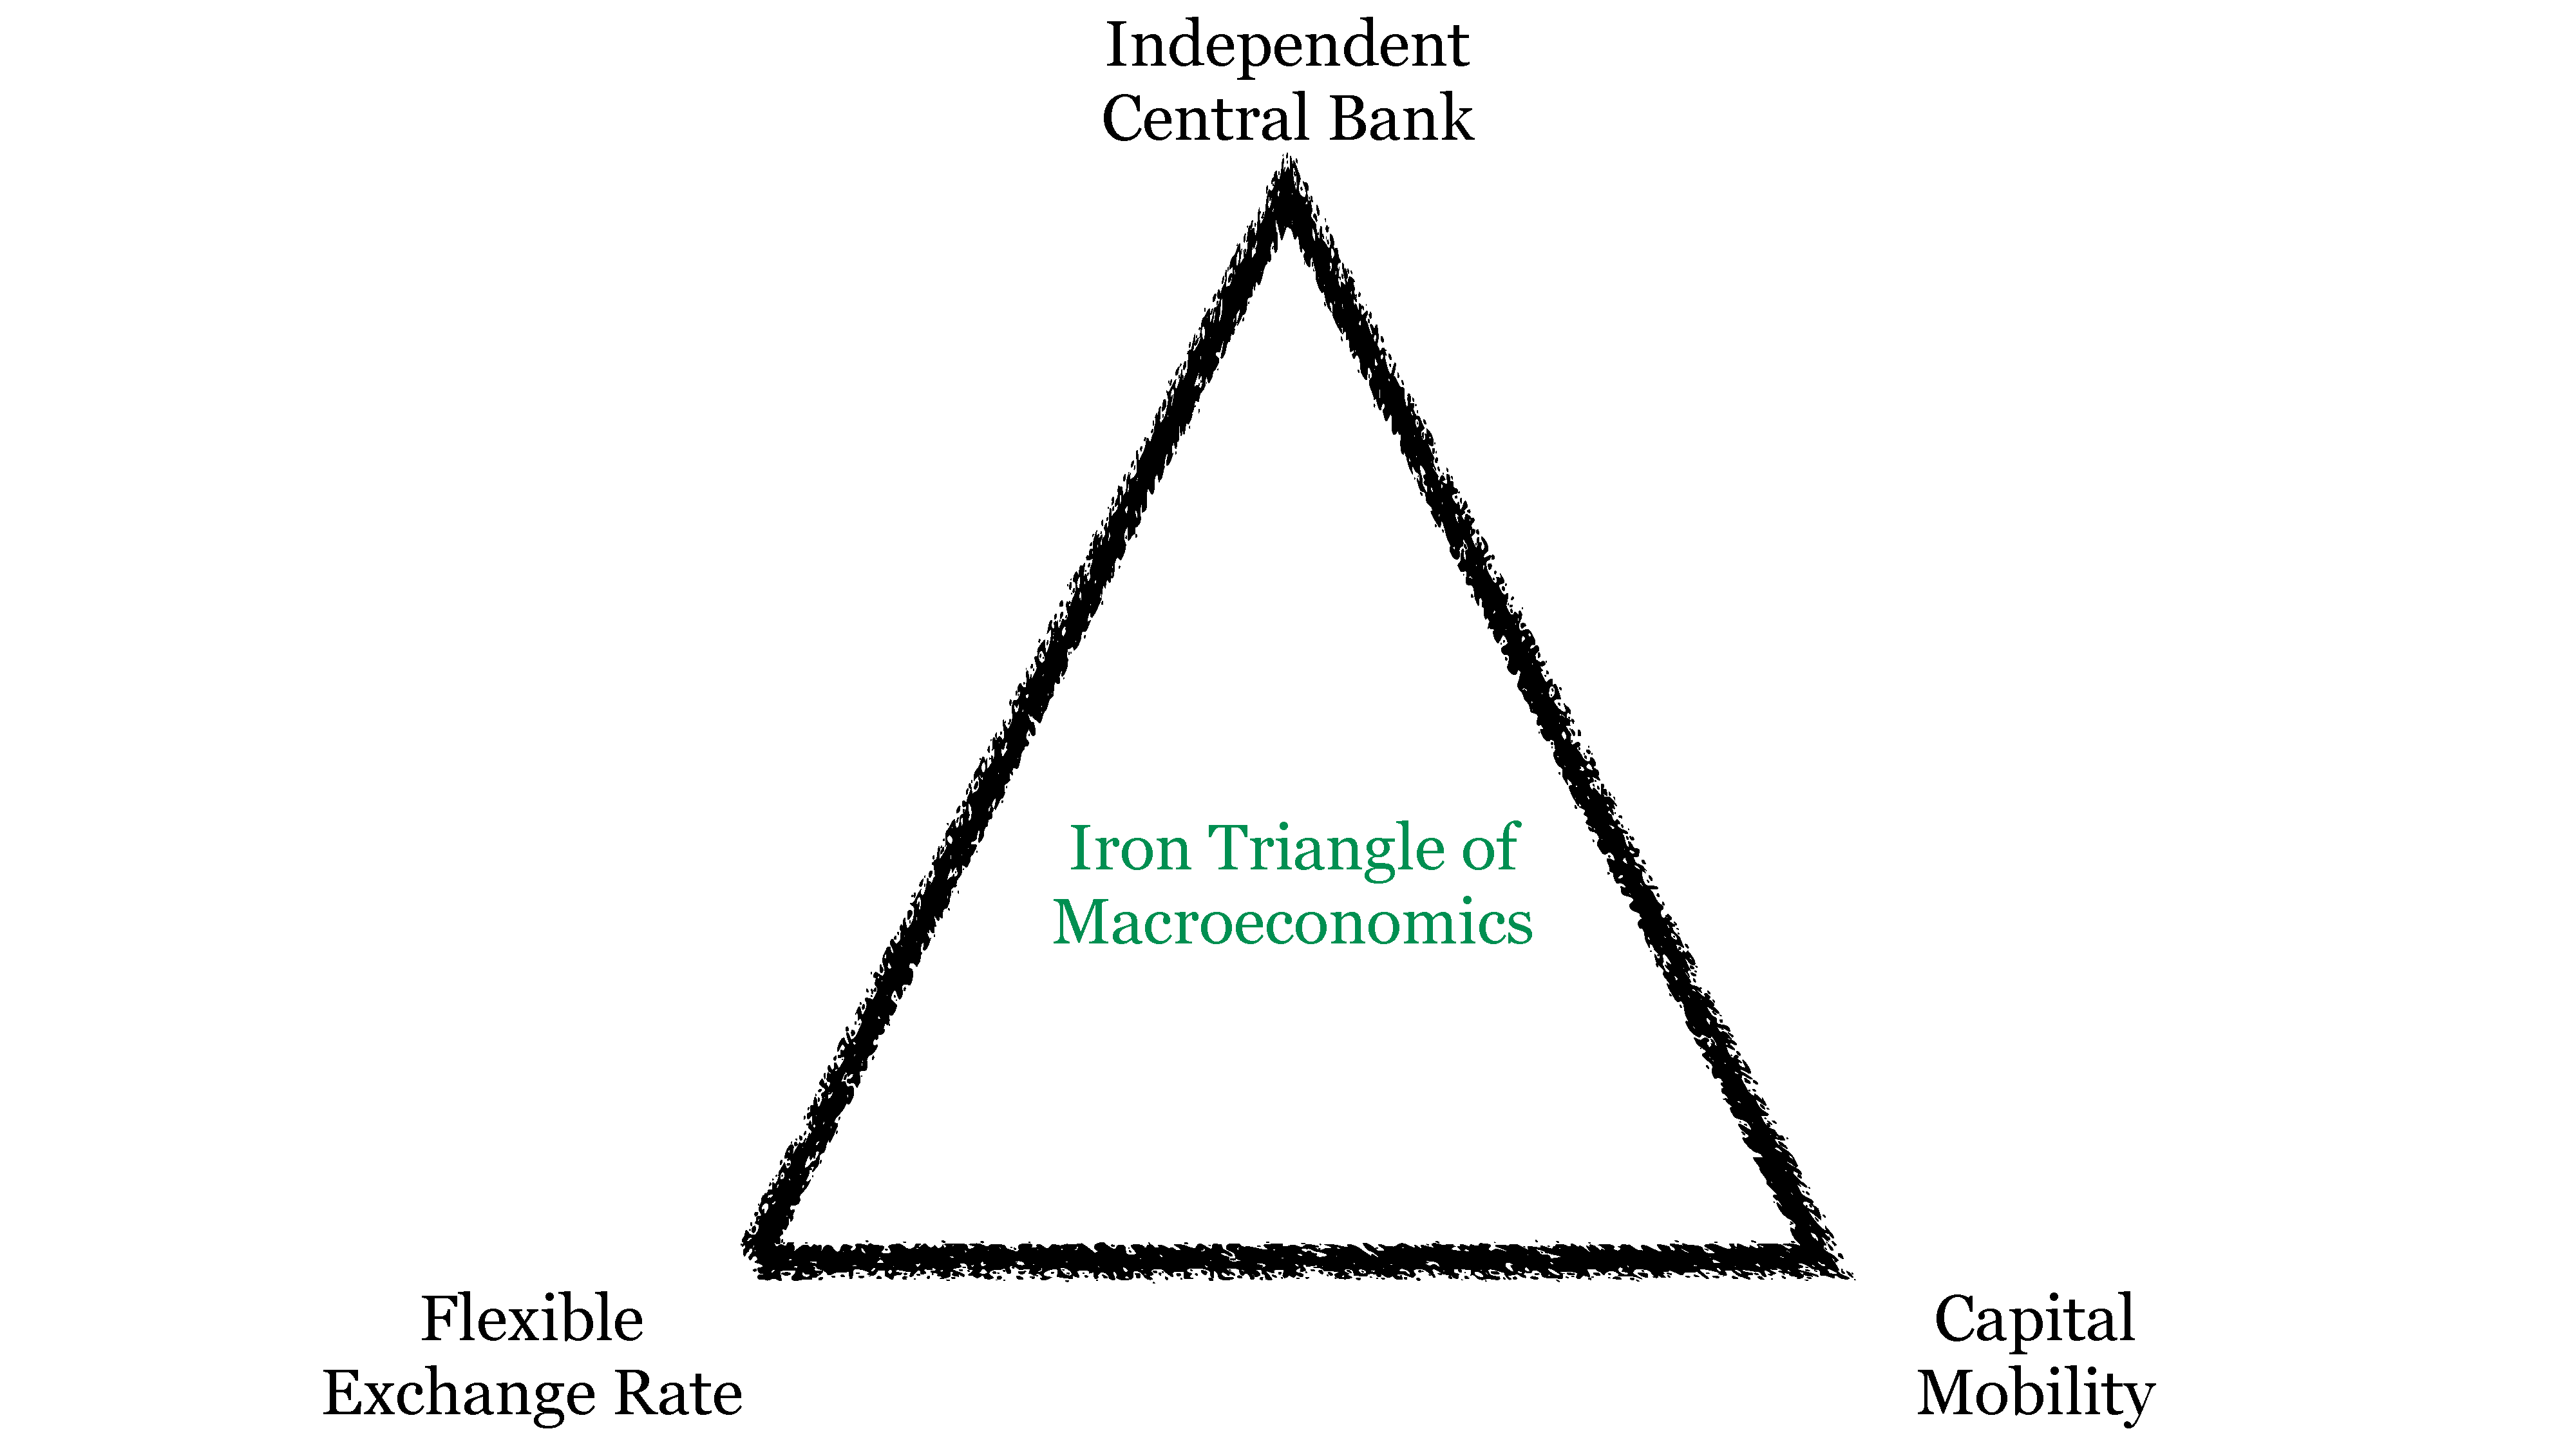
\includegraphics[width=1\linewidth]{triangle-macro}  
	\caption{The Iron Triangle of Macroeconomics}
	\label{fig:triangle-macro}
\end{figure} 

In the \gls{EU}, free capital movement is a given, and if convergence is to continue it must remain so \citep{Abiad2007}. The common market, indeed, is the minimal substrate if regional integration is to mean anything. With that corner of the impossibility triangle already occupied, \gls{EU} governments can only choose between fixed exchange rates or independent monetary policy. If governments wish to retain monetary sovereignty, they have to accept free exchange rates and any resultant volatility. If and to the extent that governments wish to limit exchange rate volatility, they \emph{must} coordinate their monetary policy, that is, enter a currency union.

\paragraph[Fiscal-CPR]{Common Pool Resource Problem.} \phantomsection \label{sec:Fiscal-CPR} If, to stabilize exchange rates, a common market must beget a common currency, to limit budget deficits, a common currency must also beget a common fiscal policy (Feldstein 2005: 7 as cited in \citealt{Begg2008}: 13). 

Without it, a common currency creates a \gls{CPR} of public debt. Inside the union, all \gls{MS} governments enjoy the low, average interest rates on its bonds. \glspl{MS} can feast on the common good of these low interest rates and take on large amounts of debt without the otherwise defining consequence of heightened interest rates as investors price in greater risk of default. %add link
Other union members may initially try to avoid any potential sovereign default, because in a highly integrated currency union, such defaults may cause systemic risks, especially with foreign union-level banks. Additionally, remaining union members may fear loss of investor confidence in the common currency if one of its members is allowed to default on its union-denominated debt. In particular, investors always worry that their sovereign bonds will be inflated away by debtor governments and therefore value a track record of sound fiscal and monetary performance not just in debtor governments, but in the entire currency, too. Currencies, in effect, are precious brands, vouching for the trustworthiness --- or lack thereof --- of the sovereign debt in which it is denominated.

Anticipating that other currency union members may want to bail out would-be sovereign defaulters, investors will downgrade the risk of any \gls{MS} debt and accept lower interest. Reacting on such incentives, \glspl{MS} may borrow more than they otherwise would or should, free-riding on the good reputation of other union members, they might eventually force to bail them out. As all currency union members face the full social cost of their sovereign debt, but the overall creditworthiness of the sum of all members naturally remains rival, choosing levels of sovereign debt at the \gls{MS} level becomes a common good: no one can be excluded from enjoying low, average interest rates, but overall solvency remains rival.

In a full fiscal union, this \gls{CPR} is resolved: the level of debt is decided at the same, highest level at which its costs eventually accrue. 

The \gls{EMU} --- seeking to counteract this moral hazard of communal interest rates --- originally forbade bail-outs, but that commitment, as it now shows, was not credible enough as Feldstein foresaw (2005: 7, as cited in \citealt{Begg2008}: 13). Absent any meaningful fiscal institutions to decide together, how much the union should raise, spend and dissave, the \gls{EMU} has fallen prey to its \gls{CPR}, or rather, its offending, extortionate, commons-exhausting members. 

%note (this is from somewhere, either Cassidy or Frank, probably frank, that more equality can make more Coase-style deals happen; that's what you want, be it in Coase-style property rights or Pigovian taxation. You don't want: having distributive stuff creep into commons et al. Good example: Pendlerpauschale in Deutschland.

%Background: Taxation Trends in the European Union

	%The Directorate General for Taxation and Customs Union issues an annual report on taxation in the European Union. Results from the 2009 edition include:
	%Tax ratios in the EU-27 remain relatively high (39.8% of GDP), but differ greatly between old and NMS (Romania 29.4%, Denmark 48.7%).
	%NMS raise relatively more revenue by indirect, non-redistributive taxes in immobile bases.
	%Almost all member states increase the (indirect) burden in (relatively immobile) consumption through VAT and excise duties. 
	%Top average (not marginal) Personal Income Tax (PIT) rates (37.8%) are in decline across almost all EU member states, but continue to vary dramatically between old and NMS (Bulgaria 10%, Denmark 59%).
	%Corporate Income Tax (CIT) rates are in rapid decline, from 35.3% in 1995 to 23.5% now. Again, NMS tend to have lower tax rates than older member states. 
	%Implicit Corporate Income Tax rates (CIT-ITR) are however, stable if diverging, possibly due to cyclical effects, base broadening or cannibalizing on the PIT.

	%Is there European (Corporate Income) Tax Competition?

	%In a liberalized Single Market, where capital and, to a lesser extent, labor through trade, investment and migration flow to their most profitable use, it appears reasonable to assume that these factors of production will also respond to taxes. Investors and workers will, as much as they can, flock to locations where tax rates are lower than the respective costs of relocation. To sustain output and growth, states would then have to compete for factors of production with low tax rates.

	%Before turning to the central question of whether this would be a desirable or undesirable dynamic, first ask whether it is real, and if so, how it came about.

	%Genschel, Kemmerling and Seils (2009) suggest (corporate income) tax competition is shaped by four interrelated institutional mechanisms of the EU:
	%Market integration (↑) reduces transaction costs of cross-border arbitrage (think: exchange rate volatility, tariffs) and thereby facilitates tax competition.
	%Enlargement (↑) adds new, attractive markets: new members are diverse in size (!) and economic development (GDP/Capita). Smaller and poorer countries have greater incentives and possibilities to lower taxes.
	%Tax coordination (↓) makes taxation more similar, and therefore reduces the ways in which governments can compete for capital and labor.
	%Supranational judicial review (↑) enforces the non-discriminatory liberalization (think: Cassis de Dijon) and limits the ability of governments to unilaterally defend against tax competition (think: Tobin Tax).

	%Genschel et al. find that tax competition is different and greater within the European Union than outside of it, and that it accelerates with time and enlargement.

	%They also suggest that larger countries suffer disproportionately from tax competition as smaller countries can boost their revenues (and growth) with the low rates on the massive inflowing capital from larger neighbors. Conversely, poorer countries have greater incentive and ease to compete for scarce capital.
	%The competition is less harsh amongst (now delegitimized) preferential tax regimes (PTR) (think: Hong Kong). When countries target only the most mobile of factors with tax breaks, the overall revenue effect tends to be smaller and more symmetric.

	%(A Prisoner's Dilemma Game of Tax Competition. Payoffs are tax revenues#.)

	%If these empirical results are correct, EU tax competition can be modeled as a Prisoner's Dilemma game, where states (strictly) dominantly prefer low taxes over high taxes and (Nash) equilibriate in suboptimal, mutual low taxation.


	%The Case against European Tax Competition: It's a Race to the Bottom

	%The argument against European tax competition builds on the assumed Prisoner's Dilemma dynamic, and suggests that EU states may not only be incapable to maximize public revenue under competition, but that thereby depressed tax revenue will lead to debt crises, the underprovision of public or common goods and impaired redistributive ability or a retrenchment of the Welfare State. It could also be argued that a harmonized European Tax regime better equips member states to withstand shocks with countercyclical tax and spend policies.

	%A related argument can be made about a presumed inability to respond to structural misalignments caused by liberalization. When trade, migration and investment allow countries to specialize even more according to their factor endowments (think: Romanian Nokia, German Management Consulting), remaining, relatively scarce factors (think: unskilled laborer in Germany) may find their market wages# fall even further below the respective socially acceptable minimum income#. Rich states may then be forced to redistribute income to these individuals, but find themselves unable to raise the necessary revenues (progressively) without further reducing their competitiveness. Tax competition could then exacerbate vicious dynamics of structural unemployment.

	%Tax competition is harshest on tax bases (capital, labor, firms) that are highly mobile (think: private equity). EU member state tax codes may be forced to converge on certain kinds of taxes. To appreciate this possibility, consider the qualities of different redistributive-/general-revenue taxes#.

	%(reproduced from Genschel 2007: 11) (whatever this was?)